\documentclass[11pt,a4paper]{article}
\usepackage[margin=2cm]{geometry}
\usepackage{lmodern}
\usepackage[T1]{fontenc}
\usepackage{amsmath,amssymb}
\usepackage{booktabs,array,tabularx,xltabular}
\usepackage{enumitem}
\usepackage{xcolor}
\usepackage[most]{tcolorbox}
\usepackage{titlesec}
\usepackage{graphicx}
\usepackage{float}
\usepackage[font=small,labelfont={bf,color=headblue},skip=4pt]{caption}
\usepackage[colorlinks=true,linkcolor=headblue,urlcolor=blue!50!black]{hyperref}

\definecolor{headblue}{RGB}{38,70,120}
\titleformat{\section}{\Large\bfseries\color{headblue}}{\thesection}{0.8em}{}[{\color{black}\titlerule}]
\titleformat{\subsection}{\large\bfseries\color{headblue}}{\thesubsection}{0.8em}{}
\titleformat{\subsubsection}{\normalsize\bfseries\color{headblue}}{\thesubsubsection}{0.8em}{}
\titlespacing*{\section}{0pt}{12pt}{6pt}
\titlespacing*{\subsection}{0pt}{9pt}{3pt}
\titlespacing*{\subsubsection}{0pt}{7pt}{2pt}
\setlength{\parindent}{0pt}
\setlength{\parskip}{5pt}
\setlist{itemsep=2pt,topsep=2pt}
\setlength{\emergencystretch}{3em}
\renewcommand{\arraystretch}{1.12}
\setlength{\tabcolsep}{4.5pt}
\setlength{\LTpre}{2pt}\setlength{\LTpost}{2pt}
\allowdisplaybreaks
\newtcolorbox{keybox}{colback=blue!3,colframe=headblue!60,boxrule=0.5pt,arc=2mm,left=2mm,right=2mm,top=1mm,bottom=1mm}
\newtcolorbox{insum}{colback=green!3,colframe=green!40!black,boxrule=0.4pt,arc=1.5mm,left=2mm,right=2mm,top=0.5mm,bottom=0.5mm,fontupper=\small}
\newcommand{\inshort}[1]{\begin{insum}\textbf{In short.} #1\end{insum}}
\newcommand{\pct}{\,\%}
\newcommand{\code}[1]{\texttt{#1}}
% title block shared by the three reports: \reporttitle{subtitle}
\newcommand{\reporttitle}[1]{%
\begin{center}
{\LARGE\bfseries\color{headblue} EV Charging with Personal and Commercial Customers\\[2pt] (Formulation 4)}\\[8pt]
{\large #1}\\[6pt]
{\normalsize CP 320 Operations Research for Mobility, course project}\\[2pt]
{\normalsize Yakshith Maddineni (SR 26080) \quad\textperiodcentered\quad Kartikeya Gaur (SR 26371)}\\[2pt]
{\normalsize 27 November 2026}
\end{center}}

\newcommand{\AMEThetaComm}{-0.33}
\newcommand{\AMEThetaPers}{12.2}
\newcommand{\BinHundred}{56{,}247}
\newcommand{\CommFCSPressure}{0.45}
\newcommand{\CommShareAll}{70.4}
\newcommand{\CommShareFree}{69.9}
\newcommand{\CommShareOfFreeVan}{7.8}
\newcommand{\CommVanHighPressPct}{98.1}
\newcommand{\CommVanPressure}{2.16}
\newcommand{\CommVanTL}{100.0}
\newcommand{\CommVanWait}{129}
\newcommand{\ConsHundred}{173{,}514}
\newcommand{\Cores}{32}
\newcommand{\CorrCommQueue}{0.13}
\newcommand{\CorrCommVan}{-0.36}
\newcommand{\CorrEPay}{0.91}
\newcommand{\CorrPersVanWithin}{0.46}
\newcommand{\CorrPressQueue}{0.35}
\newcommand{\CorrThetaComm}{-0.58}
\newcommand{\CorrThetaPercMoney}{-0.59}
\newcommand{\CorrThetaPercTime}{0.62}
\newcommand{\CorrThetaQueue}{-0.14}
\newcommand{\CorrThetaVan}{0.34}
\newcommand{\CustShareComm}{67.7}
\newcommand{\DPFcong}{7.7}
\newcommand{\DPFmax}{1130}
\newcommand{\DPFmean}{432}
\newcommand{\DPFmedian}{421}
\newcommand{\DPFoverDPM}{6}
\newcommand{\DPFperEV}{8.5}
\newcommand{\DPMmax}{333}
\newcommand{\DPMmean}{67}
\newcommand{\DeltaCOne}{146}
\newcommand{\DeltaCZero}{393}
\newcommand{\DeltaOne}{1.5}
\newcommand{\DeltaPOne}{-191}
\newcommand{\DeltaPOneDispatch}{1309}
\newcommand{\DeltaPZero}{371}
\newcommand{\DeltaZero}{0.5}
\newcommand{\DowntimeCommMid}{60.8}
\newcommand{\DowntimeCommPoor}{71.0}
\newcommand{\DowntimeCommercial}{64.3}
\newcommand{\DowntimePersonal}{60.6}
\newcommand{\DriveBottom}{2.43}
\newcommand{\DriveComm}{2.31}
\newcommand{\DrivePers}{2.03}
\newcommand{\DriveTop}{1.83}
\newcommand{\ElCF}{7.5}
\newcommand{\ElMoney}{40.2}
\newcommand{\ElMoneyComm}{30.7}
\newcommand{\ElMoneyPers}{9.5}
\newcommand{\ElOmegaComm}{15.7}
\newcommand{\ElOperator}{30.8}
\newcommand{\ElPF}{28.9}
\newcommand{\ElPFTen}{2.9}
\newcommand{\ElPiF}{15.7}
\newcommand{\ElQueueAll}{0.50}
\newcommand{\ElTariffs}{40.2}
\newcommand{\ElTime}{29.0}
\newcommand{\ElTimeComm}{16.1}
\newcommand{\ElTimePers}{12.9}
\newcommand{\ElTopFour}{10.5}
\newcommand{\ElTopFourSym}{$p^{\mathrm{M}}$}
\newcommand{\ElTopOne}{28.9}
\newcommand{\ElTopOneSym}{$p^{\mathrm{F}}$}
\newcommand{\ElTopThree}{15.7}
\newcommand{\ElTopThreeSym}{$\pi^{\mathrm{F}}$}
\newcommand{\ElTopTwo}{25.9}
\newcommand{\ElTopTwoSym}{$\mu^{C,0}$}
\newcommand{\ElVanTimePers}{2.26}
\newcommand{\ExpShareCommRich}{0.1}
\newcommand{\ExpShareCommercialUsed}{0.7}
\newcommand{\ExpSharePersFThree}{6.6}
\newcommand{\ExpSharePersRich}{27.7}
\newcommand{\ExpSharePersonalUsed}{20.8}
\newcommand{\ExpVanPiFive}{10.8}
\newcommand{\ExpVanPiNine}{2.7}
\newcommand{\ExpVanPiSeven}{6.7}
\newcommand{\ExpVanPiThree}{14.8}
\newcommand{\FreePressureMean}{0.46}
\newcommand{\FreeVanPctMean}{6.7}
\newcommand{\GapMean}{5.7}
\newcommand{\GapMed}{3.3}
\newcommand{\GreedyFoundBig}{58.9}
\newcommand{\GreedyFoundSmall}{98.2}
\newcommand{\GreedyGainBigMed}{5.3}
\newcommand{\GreedyGainMed}{3.1}
\newcommand{\GunBindCommOnCommBehind}{13.7}
\newcommand{\GunBindCommOnPersBehind}{4.9}
\newcommand{\GunBindHigh}{78.8}
\newcommand{\GunBindLow}{0.7}
\newcommand{\GunBindMedium}{6.6}
\newcommand{\GunBindPct}{13.5}
\newcommand{\GunBindPersOnCommBehind}{21.3}
\newcommand{\GunBindPersOnPersBehind}{7.8}
\newcommand{\GunBindPoorBehind}{23.7}
\newcommand{\GunBindPoorOn}{11.8}
\newcommand{\GunBindRichBehind}{2.7}
\newcommand{\GunBindRichOn}{19.2}
\newcommand{\GunMax}{40.1}
\newcommand{\GunMean}{5.1}
\newcommand{\GunMedian}{3.8}
\newcommand{\GunNCommOnCommBehind}{6003}
\newcommand{\GunNCommOnPersBehind}{1961}
\newcommand{\GunNPersOnCommBehind}{2329}
\newcommand{\GunNPersOnPersBehind}{536}
\newcommand{\InfExample}{EV-RC105\_n10}
\newcommand{\InfExampleEV}{4}
\newcommand{\InfExampleFinish}{245}
\newcommand{\InfExampleR}{151}
\newcommand{\InfExampleT}{240}
\newcommand{\InfExampleTauF}{92}
\newcommand{\InfExampleTauM}{68}
\newcommand{\InfExampleVanBack}{255}
\newcommand{\InfExampleVanEnd}{219}
\newcommand{\InfFamilies}{R1 and RC1}
\newcommand{\InfMinN}{10}
\newcommand{\InstRCOne}{80}
\newcommand{\InstROne}{120}
\newcommand{\LPDiffMax}{0.38}
\newcommand{\LPDiffMedian}{0.015}
\newcommand{\LogitAcc}{94.2}
\newcommand{\LogitBaseAcc}{93.5}
\newcommand{\LogitN}{20{,}220}
\newcommand{\LogitPseudoR}{0.45}
\newcommand{\LowVanPressure}{2.16}
\newcommand{\LowVanWait}{134}
\newcommand{\MILPExtraValid}{13}
\newcommand{\MeanThetaCommercial}{0.36}
\newcommand{\MeanThetaFCSPers}{0.64}
\newcommand{\MeanThetaPersonal}{0.69}
\newcommand{\MeanThetaVanPers}{0.89}
\newcommand{\MilpShareHigh}{21.6}
\newcommand{\MilpShareLow}{46.9}
\newcommand{\MilpShareMedium}{31.5}
\newcommand{\MipGap}{0.01}
\newcommand{\NCommVanOpt}{0}
\newcommand{\NDeadline}{24{,}870}
\newcommand{\NEVCommercial}{16{,}787}
\newcommand{\NEVPersonal}{7{,}043}
\newcommand{\NEVsValid}{23{,}830}
\newcommand{\NFCSfree}{18{,}903}
\newcommand{\NFirstNoPlan}{60}
\newcommand{\NFirstTLMajor}{50}
\newcommand{\NFreeCommercial}{14{,}125}
\newcommand{\NFreePersonal}{6{,}095}
\newcommand{\NFreeVanCommercial}{103}
\newcommand{\NFreeVanPersonal}{1214}
\newcommand{\NGreedyValid}{461}
\newcommand{\NGunLinks}{10{,}829}
\newcommand{\NInf}{51}
\newcommand{\NInfData}{51}
\newcommand{\NInst}{560}
\newcommand{\NLPPlans}{474}
\newcommand{\NLowVan}{98}
\newcommand{\NLowVanComm}{98}
\newcommand{\NLowVanOpt}{0}
\newcommand{\NNone}{35}
\newcommand{\NOpt}{277}
\newcommand{\NPatience}{18{,}903}
\newcommand{\NPressPool}{26{,}250}
\newcommand{\NPressPoolInst}{560}
\newcommand{\NQueued}{1458}
\newcommand{\NTL}{197}
\newcommand{\NValid}{474}
\newcommand{\NVans}{1040}
\newcommand{\NearLimit}{154}
\newcommand{\OmegaOne}{6}
\newcommand{\OmegaZero}{1.5}
\newcommand{\OpShareMax}{34}
\newcommand{\OpShareMin}{30}
\newcommand{\OptAtHundred}{9}
\newcommand{\OptAtTen}{55}
\newcommand{\PaidPerKWhCommercial}{17.0}
\newcommand{\PaidPerKWhPersMid}{17.1}
\newcommand{\PaidPerKWhPersTop}{19.7}
\newcommand{\PaidPerKWhPersonal}{18.2}
\newcommand{\PayCommercial}{335}
\newcommand{\PayPersonal}{352}
\newcommand{\PayShareCommercial}{69.4}
\newcommand{\PaySharePersonal}{30.6}
\newcommand{\PeakLabelHighShare}{38.7}
\newcommand{\PeakLabelShare}{32.5}
\newcommand{\PercCommercial}{582}
\newcommand{\PercPerRsCommercial}{1.74}
\newcommand{\PercPerRsPersonal}{1.88}
\newcommand{\PercPersonal}{662}
\newcommand{\PercShareCommercial}{67.7}
\newcommand{\PercSharePersonal}{32.3}
\newcommand{\PersShareOfFreeVan}{92.2}
\newcommand{\PiC}{0.70}
\newcommand{\PoolShareHigh}{32.4}
\newcommand{\PoolShareLow}{37.3}
\newcommand{\PoolShareMedium}{30.3}
\newcommand{\PressHigh}{0.6897}
\newcommand{\PressHighLoad}{20}
\newcommand{\PressLong}{0.44}
\newcommand{\PressLow}{0.1724}
\newcommand{\PressLowLoad}{5}
\newcommand{\PressShort}{0.50}
\newcommand{\QNeededHalf}{57}
\newcommand{\QNeededOne}{20}
\newcommand{\QNeededOneNoWait}{12}
\newcommand{\QNeededZero}{197}
\newcommand{\QShareBottom}{76.0}
\newcommand{\QShareComm}{91.7}
\newcommand{\QShareTop}{0.4}
\newcommand{\QueueAtLimit}{0}
\newcommand{\QueueCommercial}{1.58}
\newcommand{\QueueHigh}{5.52}
\newcommand{\QueueLow}{0.03}
\newcommand{\QueueMax}{46}
\newcommand{\QueueMaxOverW}{99.99}
\newcommand{\QueueMedium}{0.26}
\newcommand{\QueueMidComm}{1.42}
\newcommand{\QueueMidPers}{0.83}
\newcommand{\QueuePersonal}{0.41}
\newcommand{\QueuePoorCommHigh}{8.79}
\newcommand{\QueuePoorCommLow}{0.05}
\newcommand{\QueuePoorCommMedium}{0.38}
\newcommand{\QueueRichPersHigh}{0.16}
\newcommand{\QueueRichPersLow}{0.00}
\newcommand{\QueueRichPersMedium}{0.06}
\newcommand{\QueueingHigh}{30.3}
\newcommand{\QueueingLow}{0.5}
\newcommand{\QueueingMedium}{3.1}
\newcommand{\RichPersVanWait}{8}
\newcommand{\SeatsCommFree}{2.1}
\newcommand{\SeatsPersFree}{24.6}
\newcommand{\SeatsStranded}{73.3}
\newcommand{\ShortVanStopsMax}{3.0}
\newcommand{\ShortVanStopsMin}{2.5}
\newcommand{\SolveMean}{140}
\newcommand{\SolvedSamePressure}{0.48}
\newcommand{\StrandedShare}{15.1}
\newcommand{\TTCNinety}{95}
\newcommand{\TTCTen}{39}
\newcommand{\TauBarMax}{62}
\newcommand{\TauBarMin}{46}
\newcommand{\ThetaStarP}{0.66}
\newcommand{\ThetaStarPDispatch}{3.33}
\newcommand{\ThetaStarPEForty}{0.65}
\newcommand{\ThetaStarPETen}{0.67}
\newcommand{\ThetaStarPFar}{0.48}
\newcommand{\ThetaStarPNear}{0.79}
\newcommand{\ThetaStarPQten}{0.44}
\newcommand{\ThetaStarPWaitForty}{0.90}
\newcommand{\Threads}{4}
\newcommand{\TightBatt}{10.1}
\newcommand{\TightSeats}{60.4}
\newcommand{\TightTime}{29.5}
\newcommand{\TimeLimit}{300}
\newcommand{\TimeShareCommPoor}{24.8}
\newcommand{\TimeShareCommercial}{34.3}
\newcommand{\TimeShareCustComm}{34.3}
\newcommand{\TimeShareCustPers}{57.6}
\newcommand{\TimeSharePersTop}{64.7}
\newcommand{\TimeSharePersonal}{57.6}
\newcommand{\TorTopSwing}{0.39}
\newcommand{\TorTopSym}{van tariff $p^{\mathrm{M}}$}
\newcommand{\TypD}{2}
\newcommand{\TypDsaved}{12.2}
\newcommand{\TypE}{20}
\newcommand{\TypKappa}{124}
\newcommand{\TypPi}{192}
\newcommand{\TypQM}{10}
\newcommand{\TypT}{7.7}
\newcommand{\TypTauF}{54.5}
\newcommand{\TypTauM}{40}
\newcommand{\TypX}{4}
\newcommand{\UActiveShare}{80}
\newcommand{\UActiveShareLong}{80}
\newcommand{\UActiveShareShort}{81}
\newcommand{\UBattMean}{71.1}
\newcommand{\UBusyAtRHigh}{21.8}
\newcommand{\UBusyAtRLow}{6.2}
\newcommand{\UBusyAtRMedium}{23.3}
\newcommand{\UBusyHalfHigh}{26.0}
\newcommand{\UBusyHalfLow}{0.6}
\newcommand{\UBusyHalfMedium}{10.3}
\newcommand{\UChargeLong}{15.7}
\newcommand{\UChargeMean}{24.8}
\newcommand{\UChargeShort}{48.8}
\newcommand{\UEnergyFCSShare}{80.3}
\newcommand{\UEnergyPerInst}{987}
\newcommand{\UEnergyTotal}{468}
\newcommand{\UEnergyVanShare}{19.7}
\newcommand{\UFleetAll}{4.0}
\newcommand{\UFleetHundred}{69.1}
\newcommand{\UFleetMean}{43.9}
\newcommand{\UGunActiveHundred}{18.1}
\newcommand{\UGunActiveLong}{9.9}
\newcommand{\UGunActiveMean}{15.7}
\newcommand{\UGunActiveMedian}{11.4}
\newcommand{\UGunActiveShort}{23.2}
\newcommand{\UGunActiveTen}{4.6}
\newcommand{\UGunHundred}{14.5}
\newcommand{\UGunIdleShare}{29.0}
\newcommand{\UGunKWShare}{77.9}
\newcommand{\UGunLong}{7.8}
\newcommand{\UGunMean}{12.8}
\newcommand{\UGunMedian}{9.9}
\newcommand{\UGunShort}{19.4}
\newcommand{\UIdleGunsHundred}{0.3}
\newcommand{\UIdleGunsMean}{7.0}
\newcommand{\UIdleGunsTen}{18.5}
\newcommand{\UIdleShareLong}{48.1}
\newcommand{\UIdleShareMean}{38.2}
\newcommand{\UIdleShareShort}{3.3}
\newcommand{\UInstalledKW}{678}
\newcommand{\UOnRoadLong}{60.7}
\newcommand{\UOnRoadMean}{68.4}
\newcommand{\UOnRoadShort}{86.3}
\newcommand{\UPeakGunsFull}{66}
\newcommand{\UPeakGunsHundred}{17.5}
\newcommand{\UPeakGunsMax}{24}
\newcommand{\UPeakGunsMean}{12.9}
\newcommand{\UPeakVansMax}{5}
\newcommand{\UPerGunMax}{91.4}
\newcommand{\UPerGunMean}{12.8}
\newcommand{\UPerGunNinety}{34.6}
\newcommand{\UProfileLateLong}{1.3}
\newcommand{\UProfileMaxLong}{29.5}
\newcommand{\UProfileMaxShort}{50.6}
\newcommand{\UProfilePeakBinLong}{0.03}
\newcommand{\UProfilePeakBinShort}{0.43}
\newcommand{\USeatLong}{89.1}
\newcommand{\USeatMean}{79.0}
\newcommand{\USeatShort}{47.2}
\newcommand{\UStationIdleShare}{22.1}
\newcommand{\UStationMax}{81.8}
\newcommand{\UStationNinety}{33.4}
\newcommand{\USystemLong}{7.5}
\newcommand{\USystemMax}{55.7}
\newcommand{\USystemMean}{12.4}
\newcommand{\USystemShort}{18.7}
\newcommand{\UVanDelivShare}{83.2}
\newcommand{\UVanDriveShare}{7.6}
\newcommand{\UVanEnergyCheck}{0.01}
\newcommand{\UVanLossShare}{9.2}
\newcommand{\UnsolvedFamilies}{C1, C2, R1, RC1, RC2}
\newcommand{\UnsolvedMinN}{60}
\newcommand{\UnsolvedPressure}{1.35}
\newcommand{\UserShareBottom}{49.2}
\newcommand{\UserShareComm}{74.2}
\newcommand{\UserShareTop}{8.3}
\newcommand{\ValidNoWarm}{13}
\newcommand{\ValidRCOne}{42}
\newcommand{\ValidROne}{75}
\newcommand{\VanBindPct}{38.7}
\newcommand{\VanCommHigh}{3.4}
\newcommand{\VanCommLow}{0.0}
\newcommand{\VanCommMedium}{0.0}
\newcommand{\VanCommOpt}{0.0}
\newcommand{\VanCommOptMax}{0.0}
\newcommand{\VanDualMean}{5.5}
\newcommand{\VanPctMean}{21}
\newcommand{\VanPersBelowFour}{0.0}
\newcommand{\VanPersEightNine}{28.0}
\newcommand{\VanPersHigh}{16.6}
\newcommand{\VanPersLow}{23.4}
\newcommand{\VanPersMedium}{17.1}
\newcommand{\VanPersNineTen}{50.2}
\newcommand{\VanPersOpt}{19.3}
\newcommand{\VanPersSixSeven}{6.6}
\newcommand{\VanRichPersHigh}{32.7}
\newcommand{\VanRichPersLow}{50.0}
\newcommand{\VanRichPersMedium}{33.1}
\newcommand{\VanShareCommercial}{0.7}
\newcommand{\VanSharePersonal}{19.9}
\newcommand{\VanStopsCOne}{5.7}
\newcommand{\VanStopsCTwo}{5.5}
\newcommand{\VanStopsRCOne}{2.5}
\newcommand{\VanStopsRCTwo}{4.9}
\newcommand{\VanStopsROne}{3.0}
\newcommand{\VanStopsRTwo}{5.6}
\newcommand{\VanTopCommercialLong}{--}
\newcommand{\VanTopCommercialShort}{0.0}
\newcommand{\VanTopPersonalLong}{41.9}
\newcommand{\VanTopPersonalShort}{39.1}
\newcommand{\VanWaitZeroShare}{54}
\newcommand{\VansFull}{48.1}
\newcommand{\VansMean}{2.2}
\newcommand{\WCommOne}{15}
\newcommand{\WCommZero}{40}
\newcommand{\WarmCost}{453}
\newcommand{\WarmFinish}{8}
\newcommand{\WarmNone}{99}
\newcommand{\Workers}{8}
\newcommand{\ZCustomer}{69.2}
\newcommand{\ZFive}{39.3}
\newcommand{\ZFour}{20.9}
\newcommand{\ZOne}{0.9}
\newcommand{\ZOperator}{30.8}
\newcommand{\ZRecMax}{0.38}
\newcommand{\ZSix}{29.0}
\newcommand{\ZThree}{7.5}
\newcommand{\ZTwo}{2.4}
\newcommand{\ZperMax}{1103}
\newcommand{\ZperMean}{885}
\newcommand{\ZperMin}{769}
\newcommand{\ZperRCOneMean}{1036}
\newcommand{\ZperRTwoMean}{817}

\newtcolorbox{keyboxb}{breakable,colback=blue!3,colframe=headblue!60,boxrule=0.5pt,arc=2mm,left=2mm,right=2mm,top=1mm,bottom=1mm}

\begin{document}
\sloppy

\reporttitle{Comprehensive MILP report: assumptions, exploratory analysis, shadow prices and sensitivity}

\begin{keybox}
{\color{headblue}\textbf{How to read this report}}\\
This report covers the exact solver (MILP, Gurobi) of formulation~4 on the baseline settings. Formulation~4 is formulation~3 with one more customer attribute: every EV is a \emph{personal} car or a \emph{commercial} car (taxi, ride-hailing, fleet), and each segment has its own income distribution and its own money and time sensitivities. The report has three parts. \textbf{Part I} lists every assumption behind the model, the data and the run, with the reason for each and what changes if it is relaxed. \textbf{Part II} is an exploratory analysis of the \NInst{} instances and the \NValid{} valid plans. \textbf{Part III} analyses the results point by point: the anatomy of the objective, the shadow prices (dual values) of the plans, the income threshold of each segment predicted by theory, the choice of resource, queues, peak demand, horizons, infrastructure utilisation, the vans, equity, computation, infeasibility and sensitivity to the income distributions and the segment mix. Every subsection ends with a green \emph{In short} box. Section~\ref{sec:glossary} explains every technical term. The RL method and the experiments E1--E8 have their own reports.
\end{keybox}

\begin{keyboxb}
{\color{headblue}\textbf{The main results in eleven lines}}
\begin{enumerate}[leftmargin=1.4em,itemsep=1pt]
  \item \NOpt{} instances are solved to optimality and \NTL{} more end at the time limit with a valid plan (median gap \GapMed\pct); all \NInf{} infeasible instances are infeasible because of the data alone (Sections~\ref{sec:eda}, \ref{sec:infeasible}).
  \item Vans go to personal cars: \VanSharePersonal\pct{} of free-choice personal EVs get a van against \VanShareCommercial\pct{} of commercial EVs, although commercial EVs are \CommShareFree\pct{} of all free-choice EVs (Section~\ref{sec:choice}).
  \item In proven-optimal plans \emph{no} commercial free-choice EV gets a van; the \NFreeVanCommercial{} that do are all in time-limit plans, \CommVanHighPressPct\pct{} of them at high demand pressure, and wait \CommVanWait{} min for the van on average (Section~\ref{sec:choice}).
  \item Theory explains why: for a typical commercial EV the van costs \DeltaCOne{} Rs more than the station even at $\theta=1$; it only pays off behind a station queue of at least \QNeededOne{} minutes, longer than a rich driver's queue tolerance (Section~\ref{sec:threshold}).
  \item For personal EVs theory predicts the income threshold $\theta^{*}=\ThetaStarP$; in optimal plans no personal EV below $\theta=0.4$ gets a van and the share rises to \VanPersNineTen\pct{} at $\theta$ 0.9--1.0 (Section~\ref{sec:threshold}).
  \item Commercial drivers do \QShareComm\pct{} of all queueing at stations while they are \UserShareComm\pct{} of the station users; the poorest 40\pct{} of station users do \QShareBottom\pct{} of it (Section~\ref{sec:queues}).
  \item A gun-minute is worth \GunMean{} Rs on average when it is scarce; a link is binding most often when a personal EV holds the gun and a commercial EV waits behind it (\GunBindPersOnCommBehind\pct) (Section~\ref{sec:duals}).
  \item Patience limits and the deadline $T$ have zero shadow price in every plan; one more kW of station-gun power is worth about \DPFmean{} Rs per instance, \DPFoverDPM{} times a kW of van power (Section~\ref{sec:duals}).
  \item $Z$ is most sensitive to the station tariff $p^{\mathrm F}$ (elasticity \ElPF\pct) and the money sensitivity of low-income commercial drivers (\ElTopTwo\pct): commercial customers carry \CustShareComm\pct{} of the perceived cost (Section~\ref{sec:anatomy}).
  \item The segment mix is a first-order input: with $\pi_{\mathrm C}=0.3$ instead of \PiC{} the expected van share of free-choice EVs would be \ExpVanPiThree\pct{} instead of \ExpVanPiSeven\pct{} (Section~\ref{sec:sensitivity}).
  \item The infrastructure is sized for the peak: guns are busy \UGunMean\pct{} of $[0,T]$ on average (\UGunShort\pct{} with short, \UGunLong\pct{} with long horizons), the whole installed power is used \USystemMean\pct, and the dispatched vans charge only \UChargeMean\pct{} of $T$; yet all 24 guns are busy at once in \UPeakGunsFull{} plans (Section~\ref{sec:util}).
\end{enumerate}
\end{keyboxb}

\tableofcontents
\newpage

%=====================================================================
\section{Glossary}
\label{sec:glossary}

\begin{xltabular}{\textwidth}{@{}>{\raggedright\arraybackslash}p{4.0cm}X@{}}
\toprule
\textbf{Term} & \textbf{Meaning} \\
\midrule
\endhead
EV & Electric vehicle that asks to be charged during the planning period. \\
FCS, gun & Fixed charging station; each has 2 \emph{guns} (charging points) of 22\,kW. A gun charges one EV at a time. \\
MCS, van & Mobile charging station: a van with a 150\,kWh battery that drives to parked EVs and charges them one at a time at 30\,kW, starting and ending at the depot. \\
Request time $r_i$ & Minute at which EV $i$ asks for charging. \\
Horizon $T$ & Length of the planning period in minutes; every EV must be fully charged and every van back by $T$. \\
Stranded EV & EV whose remaining range is shorter than the distance to the nearest station; it can only be served by a van. \\
Free-choice EV & EV with at least one station in range; the model really chooses between station and van for it. \\
Use segment $s_i$ & \textbf{Personal} (P): a private car; its time cost depends on where the driver is. \textbf{Commercial} (C): taxi, ride-hailing or fleet car; every minute out of service is lost earnings. \\
Commercial share $\pi_{\mathrm C}$ & Probability that an EV is commercial; \PiC{} in the data (share of commercial cars among \emph{public charging requests}). \\
Income index $\theta_i$ & Number in $[0,1]$ giving the household's position in the urban income distribution: 0 = lowest, 1 = highest. Drawn per segment: Beta(2.5,\,1) for personal, Beta(3,\,5) for commercial EVs. \\
Income band / decile & Groups of $\theta$: bands of width 0.2 (0.0--0.2, \dots), deciles of width 0.1. \\
Money sensitivity $\mu^{s}(\theta)$ & How strongly a customer feels one rupee paid; falls with income. \\
Value of time $c^{a,s}(\theta)$ & Rupees per minute a customer would pay to save a minute of activity $a$: D driving, Q queueing, C charging at a station, V waiting for and being charged by a van. Rises with income. Written $c^{a,s,0}$ and $c^{a,s,1}$ at $\theta=0$ and $\theta=1$. \\
Downtime, downtime rate $\omega(\theta)$ & For a commercial EV the time from request to full charge, during which it earns nothing. Every downtime minute costs $\omega(\theta)=c^{\mathrm D,\mathrm C}=c^{\mathrm C,\mathrm C}=c^{\mathrm V,\mathrm C}$; a queue minute costs $\omega+\delta$. \\
Driver-free benefit & A personal driver is free while a van charges the parked car, so van minutes cost $c^{\mathrm V,\mathrm P}<c^{\mathrm C,\mathrm P}$. A taxi has no such benefit: a parked taxi earns nothing either way. \\
Queue tolerance $W^{s}(\theta)$ & Longest queue (minutes) a customer accepts at a station; falls with income. \\
Tariff $p^{\mathrm F}$, $p^{\mathrm M}$ & Price per kWh the customer pays at a station and for the van service; the same for both segments. \\
Perceived cost & Money paid weighted by $\mu_i$ plus time weighted by the values of time: what the customer \emph{feels}. \\
Operator cost & Van driving, van dispatch and energy: what the operator pays. \\
Objective $Z$ & Operator cost plus perceived customer cost, summed over all EVs; the model minimises it. \\
MILP & Mixed-integer linear program: an optimisation model with linear constraints, some variables restricted to 0/1. \\
Binary variable & Variable that is 0 or 1, used for yes/no decisions (``EV $i$ on gun $g$''). \\
Big-$M$ constraint & Constraint switched on or off by a binary variable through a large constant $M$. \\
LP relaxation & The MILP with the 0/1 restrictions dropped; its optimum is a lower bound on $Z$. \\
Branch and bound (B\&B) & The method Gurobi uses: it splits the problem on binary variables and prunes parts whose bound is worse than the best plan found. \\
Best bound, MIP gap & Best bound = lowest $Z$ any plan could still have. Gap = (plan $Z$ $-$ bound)/plan $Z$. Gap 0 = proven optimal. \\
Optimal plan & Plan proven optimal by Gurobi within the time limit. \\
Time-limit plan & Valid plan found when the time ran out, not proven optimal. \\
Infeasible & No plan can satisfy all constraints. \\
Unsolved & Gurobi found no plan in the time limit but did not prove infeasibility either. \\
Warm start, greedy plan & A simple feasible plan built rule by rule and handed to Gurobi as a starting point. \\
Independent checker & Separate code that tests every constraint of a plan and recomputes $Z$ from scratch. \\
Dual variable, shadow price & For a linear program, the change of the optimal objective when the right-hand side of one constraint grows by one unit. Here in Rs per minute or per kW. \\
Binding constraint & Constraint that holds with equality at the optimum; only binding constraints can have non-zero shadow prices. \\
Complementary slackness & LP rule: a constraint with slack (not binding) has shadow price zero, and vice versa. \\
Degenerate & An optimum where more constraints are binding than needed; the shadow prices are then not unique. \\
Fixed-plan LP & The LP left after fixing all yes/no decisions of a plan; used here to obtain shadow prices. \\
Envelope theorem & The derivative of the optimal objective with respect to a cost coefficient equals the quantity that coefficient multiplies in the optimal plan. \\
Elasticity & Percentage change of $Z$ for a 1\pct{} change of a coefficient. \\
Demand pressure & $\text{load}_i/29$: the number of EVs of the instance (EV $i$ included) whose request falls in the window of one mean station charging time before $r_i$, divided by the 29 chargers (24 guns + 5 vans). Data only, the same in all three reports (Section~\ref{sec:defs}). \\
Pressure tercile & Low $\le\PressLow$, medium, high $>\PressHigh$ (load $\le\PressLowLoad$, $>\PressHighLoad$): cut points pooled over the free-choice EVs of all \NPressPoolInst{} baseline instances, so an EV has the same tercile in every report. \\
Utilisation & Share of an available resource that is used: busy minutes over $[0,T]$ for a gun, stops over 6 seats or kWh drawn over 150\,kWh for a van, energy delivered over installed power $\times\,T$ for the system (Section~\ref{sec:util}). \\
Tercile & Split into three equal-sized groups (low, medium, high). \\
Wilson interval & 95\pct{} confidence interval for a share; more reliable than the usual $\pm1.96\,\sigma$ for small or extreme shares. \\
Logistic regression & Statistical model of the probability of a yes/no outcome (here ``served by a van'') as a function of several factors. \\
Average marginal effect (AME) & Average change in that probability when one factor rises by a given amount. \\
Spearman correlation & Correlation of the ranks of two variables; $-1$ to $+1$; robust to outliers. \\
Beta($a,b$) & Family of distributions on $[0,1]$; $a=b$ is symmetric, $a=b=1$ uniform, $a<b$ leans to low values, $a>b$ to high values. \\
Solomon instance, family & Classic vehicle-routing test data. Families C (clustered), R (random), RC (mixed) with type 1 (short horizon) and type 2 (long horizon). \\
Peak / off-peak & Busy / calm times; measured here by demand pressure. \\
\bottomrule
\end{xltabular}

%=====================================================================
\clearpage
\part{Assumptions}
\section{All assumptions behind the results}
\label{sec:assumptions}

\subsection{The problem in one paragraph}
During a planning period $[0,T]$ parked EVs request charging. Each request is served by exactly one resource: the EV drives to a fixed station (FCS) and charges at one of its guns, or a van (MCS) drives to the EV and charges it in place. The model decides who is served where, the order on every gun, the route of every van and every start time. It minimises the operator's cost plus the cost each customer perceives. Every customer has a use segment (personal or commercial) and an income index $\theta_i$; both change how a rupee and a minute are felt. The model is formulation~4 (\texttt{formulation\_4.pdf}): the variables and constraints (1)--(23) of formulation~3, with segment-dependent coefficients, so the MILP has exactly the size of formulation~3.

\subsection{Modelling assumptions}
\begin{xltabular}{\textwidth}{@{}>{\raggedright\arraybackslash}p{4.6cm}>{\raggedright\arraybackslash}p{5.2cm}X@{}}
\toprule
\textbf{Assumption} & \textbf{Why} & \textbf{What changes if relaxed} \\
\midrule
\endhead
All requests are known at time 0 (offline planning). & Gives the best possible plan, a benchmark for any real-time rule. & Real-time (online) planning would do worse; the gap is the value of information. \\
Every EV must be fully charged by $T$ (hard). & The brief asks that all requests be served. & Allowing partial charging or late completion would turn the \NInf{} infeasible instances into feasible ones with a penalty. \\
An FCS user drives there on its own battery and stays until charged. & How public charging works. & Leaving early or partial charging would shorten gun times and queues. \\
EVs can only reach stations within their remaining range. & Physical limit. & Without it there would be no stranded EVs and vans would rarely leave the depot (Section~\ref{sec:threshold}). \\
A van user stays parked; the van comes to it. & Defines the van service. & --- \\
One EV per gun and per van at a time, no pre-emption. & Equipment limit. & Sharing power between EVs would change the timing constraints. \\
Van driving and delivered energy share one battery; no recharging of the van during the period. & Simplest van energy model. & Recharging would remove the battery limit (it is the tightest van resource in only \TightBatt\pct{} of vans, Section~\ref{sec:vans}). \\
Constant charging power. & Linear model. & Real charging slows above about 80\pct{} state of charge; times would grow. \\
\textbf{(F4)} Every customer has a use segment $s_i$ and an income index $\theta_i$, both known in advance; $(s_i,\theta_i)$ drawn independently per EV. & Market segmentation by a discrete and a continuous attribute (professor's suggestion, extended in Section~4.14 of the formulation-3 report). & With unknown attributes the operator would plan for an average customer. \\
\textbf{(F4)} The attributes act only through $\mu^{s}(\theta)$, $c^{a,s}(\theta)$ and $W^{s}(\theta)$, straight lines in $\theta$ with their own end points per segment. & Keeps the model linear and the effect transparent. & Other channels (car type, home charger, shift patterns) would need more attributes. \\
\textbf{(F4)} A commercial car's time is its downtime: driving, charging and van time all cost $\omega(\theta)$, queueing $\omega+\delta$. & A parked taxi earns nothing whatever the driver does. & With a driver-free discount for taxis too, commercial EVs would value vans like personal ones (Section~\ref{sec:threshold}). \\
\textbf{(F4)} The segment changes no network data; both segments pay the same tariffs. & Any difference between segments then comes only from the sensitivities and the income distributions. & Segment-specific tariffs (fleet contracts) would shift the commercial threshold directly. \\
Customers pay $p^{\mathrm F}$ at a station and $p^{\mathrm M}\ge p^{\mathrm F}$ for the van. & The van is a premium door-step service. & Equal tariffs would remove the money reason for low incomes to avoid vans (experiment E1). \\
The operator minimises its cost plus the customers' perceived cost; tariff revenue is not a gain. & System view: an operator that cares about its customers. & A profit-maximising operator would push customers to the dearer van. \\
\bottomrule
\end{xltabular}

\subsection{Network, time and demand data (EV-Solomon)}
\begin{xltabular}{\textwidth}{@{}>{\raggedright\arraybackslash}p{4.6cm}>{\raggedright\arraybackslash}p{4.0cm}X@{}}
\toprule
\textbf{Item} & \textbf{Value} & \textbf{Source / reason} \\
\midrule
\endhead
Instances & 56 Solomon files, first $n=10,20,\dots,100$ EVs & Classic benchmark; ``first $n$'' is Solomon's own convention. \\
Locations & Solomon coordinates; 1 grid unit = 0.2\,km & A $100\times100$ grid becomes a $20\times20$\,km city. \\
Road distance & $1.3\times$ straight line & Usual detour factor of city roads. \\
Speed & 15.6\,km/h & Chosen so that travel minutes equal Solomon's grid distance (Solomon's rule); evening city traffic. \\
Horizon $T$ & Solomon depot due date: C1 1236, C2 3390, R1 230, R2 1000, RC1 240, RC2 960 min & Unchanged from Solomon (never extended). \\
Request time $r_i$ & Solomon ready time & Unchanged; only these differ within a family. \\
Energy demand $E_i$ & Solomon demand 1--50 mapped linearly to 10--40\,kWh & Typical top-up of a city EV. \\
Remaining range $R_i$ & Uniform 5--40\,km; \StrandedShare\pct{} of EVs stranded & Creates EVs that only a van can serve. \\
Stations & 12 (k-means centres of the EVs), 2 guns of 22\,kW & Stations placed where demand is. \\
Vans & 5; battery 150\,kWh; 30\,kW; at most $Q_m=6$ EVs; 0.25\,kWh/km; 90\pct{} transfer efficiency & Typical mobile charger. \\
\textbf{(F4)} Segment $s_i$ & Commercial with probability $\pi_{\mathrm C}=\PiC$; \CommShareAll\pct{} of the EVs in valid plans are commercial & \texttt{data/calibration.md}: commercial cars are about 10\pct{} of e-car registrations but drive far more and charge in public far more often, so they dominate public charging requests. \\
\textbf{(F4)} Income $\theta_i$ & personal Beta(2.5,\,1), mean \MeanThetaPersonal; commercial Beta(3,\,5), mean \MeanThetaCommercial & Car ownership by urban income quintile (HCES) for personal owners; cab-driver earnings surveys for commercial drivers. \\
Same EVs within a family & Positions, energies, ranges, $s_i$ and $\theta_i$ identical in a family & Files of a family differ only in request times. \\
\bottomrule
\end{xltabular}

\subsection{Cost and price parameters}
\begin{xltabular}{\textwidth}{@{}>{\raggedright\arraybackslash}p{2.6cm}>{\raggedright\arraybackslash}p{2.0cm}>{\raggedright\arraybackslash}p{4.6cm}X@{}}
\toprule
\textbf{Parameter} & \textbf{Value} & \textbf{Meaning} & \textbf{Effect of a higher value} \\
\midrule
\endhead
$c^{\mathrm{EV}}$ & 4 Rs/km & cost of driving an EV to a station (customer pays) & stations far away less attractive; more vans for distant EVs \\
$c^{\mathrm M}$ & 15 Rs/km & van driving cost & shorter van routes; fewer detours to free-choice EVs \\
$c^{\mathrm F}_m$ & 1500 Rs & fixed cost of sending out a van & fewer vans; vans leave only for stranded EVs \\
$\pi^{\mathrm F}$ & 8.7 Rs/kWh & operator's grid energy at a station & stations dearer for the operator; vans relatively cheaper \\
$\pi^{\mathrm M}$ & 10.7 Rs/kWh & operator's van battery energy (lost 10\pct{} in transfer) & vans dearer; thresholds rise \\
$p^{\mathrm F}$ & 15 Rs/kWh & station tariff (customer) & raises everybody's cost at a station \\
$p^{\mathrm M}$ & 25 Rs/kWh & van tariff (customer) & the van premium hurts low incomes; thresholds rise \\
\bottomrule
\end{xltabular}

\subsection{Customer parameters per segment}
\begin{table}[H]
\centering\small
\caption{Customer parameters of the run (straight lines between $\theta=0$ and $\theta=1$, per segment; \texttt{common/f4\_params.json}).}
\label{tab:params}
\begin{tabular}{llrrrr}\toprule
 & & \multicolumn{2}{c}{personal} & \multicolumn{2}{c}{commercial} \\
\cmidrule(lr){3-4}\cmidrule(lr){5-6} parameter & unit & $\theta=0$ & $\theta=1$ & $\theta=0$ & $\theta=1$ \\ \midrule
income $\theta$ given the segment & -- & \multicolumn{2}{c}{Beta(2.5, 1)} & \multicolumn{2}{c}{Beta(3, 5)} \\
money sensitivity $\mu$ & Rs/Rs & 1.5 & 0.5 & 1.5 & 0.5 \\
value of time $c^{\mathrm{D}}$ (driving to an FCS) & Rs/min & 1.5 & 15 & 1.5 & 6 \\
value of time $c^{\mathrm{Q}}$ (queueing at an FCS) & Rs/min & 2.5 & 25 & 2 & 7.5 \\
value of time $c^{\mathrm{C}}$ (charging at an FCS) & Rs/min & 1 & 10 & 1.5 & 6 \\
value of time $c^{\mathrm{V}}$ (van wait + van charging) & Rs/min & 0.5 & 5 & 1.5 & 6 \\
queue tolerance $W$ & min & 60 & 15 & 40 & 15 \\
tariff $p^{\mathrm{F}}$ / $p^{\mathrm{M}}$ (both segments) & Rs/kWh & \multicolumn{4}{c}{15 / 25} \\
\bottomrule\end{tabular}

\end{table}
\begin{itemize}
  \item \textbf{Personal} lines are those of formulation~3: queueing dearer than driving, van minutes ($c^{\mathrm V}$) cheaper than station-charging minutes ($c^{\mathrm C}$) because the driver is free.
  \item \textbf{Commercial} lines: one downtime rate $\omega(\theta)$ from \OmegaZero{} to \OmegaOne{} Rs/min for driving, charging and the van; queueing costs $\delta$ = \DeltaZero{} to \DeltaOne{} Rs/min more. The money sensitivity is the same as for personal customers (a rupee is felt according to household income). The commercial queue tolerance is shorter at low income (every minute is lost earnings).
  \item The segment share and the two income distributions are calibrated from Indian data (\texttt{data/calibration.md}); all other end points are placeholders chosen by us. Section~\ref{sec:calibration} lists sources that could replace them.
\end{itemize}

\subsection{Solver and run settings}
\begin{itemize}
  \item Gurobi 13, complete model (no reduced model), time limit \TimeLimit\,s per instance, MIP gap target \MipGap\pct, \Workers{} instances at a time with \Threads{} threads each (\Cores{} cores) on the lab server.
  \item Every instance was given to Gurobi; nothing was skipped beforehand. A greedy plan was offered as a warm start when one existed.
  \item Every plan was checked by the independent checker (\texttt{common/check\_plan\_f4.py}), which recomputes $Z$ from scratch.
\end{itemize}

\subsection{Definitions used in the analysis}
\label{sec:defs}
\begin{itemize}
  \item Shares of ``served by a van'' are over free-choice EVs only; stranded EVs take a van whatever their segment or income.
  \item \textbf{Demand pressure} (one definition for the three reports, \texttt{common/infra.py}). For an instance (a file and its first $n$ EVs):
  \begin{gather*}
  \text{window}=\frac1n\sum_{j}\frac{60E_j}{22\text{ kW}},\qquad
  \text{pressure}_i=\frac{\text{load}_i}{24\text{ guns}+5\text{ vans}},\\
  \text{load}_i=\#\{j:\ r_i-\text{window}\le r_j\le r_i\}\quad(i\text{ included}).
  \end{gather*}
  The window is \TauBarMin--\TauBarMax{} min. Pressure uses only the data (request times, energies, fleet), never a plan, so an EV has the same pressure in every method and variant. \textbf{Terciles:} cut points at the 1/3 and 2/3 quantiles of pressure over the \NPressPool{} free-choice EVs of all \NPressPoolInst{} baseline instances (feasible or not): low $\le\PressLow$ (load $\le\PressLowLoad$), medium, high $>\PressHigh$ (load $>\PressHighLoad$). Because load is an integer the groups are not exactly equal (\PoolShareLow, \PoolShareMedium{} and \PoolShareHigh\pct{} of the pool); among the free-choice EVs of the valid MILP plans they are \MilpShareLow, \MilpShareMedium{} and \MilpShareHigh\pct{} (the unsolved and infeasible instances are the congested ones).
  \item What pressure ignores: travel time to the station, charging still in progress from earlier requests (only arrivals inside one window count), and the difference between a gun and a van (a van counts as one charger). Formulation~4's own peak/off-peak label (\texttt{period}: peak if $\text{load}_i$ is above the instance's median load) is a different, coarser, instance-relative measure: it marks \PeakLabelShare\pct{} of the pooled free-choice EVs as peak, and only \PeakLabelHighShare\pct{} of those are in the high tercile. This report uses the terciles throughout.
  \item Shadow prices come from the fixed-plan LP of each plan (Section~\ref{sec:duals}); they hold \emph{for the given decisions}.
  \item The analysis files are built by \texttt{prepare\_data\_f4.py} from \texttt{baseline\_MILP/results} (\texttt{runs.csv}, \texttt{plan.csv}) and the formulation-4 data.
\end{itemize}

\inshort{Fifteen modelling assumptions (four new in formulation~4), thirteen data choices, seven cost parameters, two sets of customer lines and the solver settings define every result below. The segment share and the income distributions are calibrated; the money and time lines are placeholders whose directions come from the formulation and whose sizes set the results.}

%=====================================================================
\clearpage
\part{Results: exploratory analysis}
\section{Exploratory analysis of the results}
\label{sec:eda}

\subsection{How the instances ended}
\begin{figure}[H]
\centering
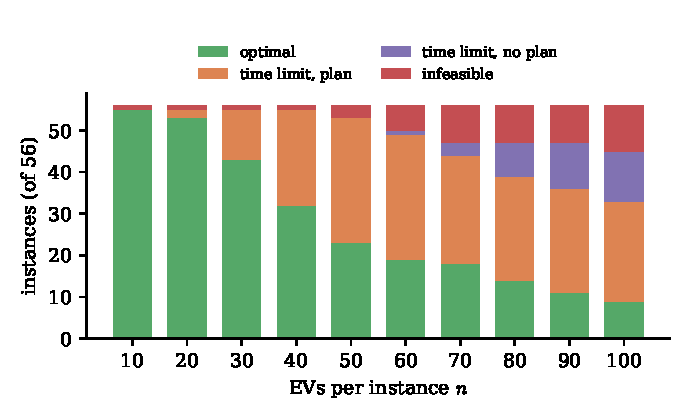
\includegraphics[width=0.62\textwidth]{figures/solver_outcome.pdf}
\caption{Outcome of the 56 instances of each size.}
\label{fig:solver}
\end{figure}
\begin{table}[H]
\centering\small
\caption{Solver outcome per instance size; gap of the time-limit plans.}
\label{tab:solver}
\begin{tabular}{lrrrrrrr}\toprule
$n$ & instances & optimal & \shortstack{time limit\\with plan} & \shortstack{time limit\\no plan} & infeasible & \shortstack{median\\gap (\%)} & \shortstack{mean\\time (s)} \\ \midrule
10 & 56 & 55 & 0 & 0 & 1 & -- & 0 \\
20 & 56 & 53 & 2 & 0 & 1 & 2.05 & 19 \\
30 & 56 & 43 & 12 & 0 & 1 & 1.65 & 83 \\
40 & 56 & 32 & 23 & 0 & 1 & 2.75 & 139 \\
50 & 56 & 23 & 30 & 0 & 3 & 5.33 & 170 \\
60 & 56 & 19 & 30 & 1 & 6 & 6.29 & 176 \\
70 & 56 & 18 & 26 & 3 & 9 & 6.02 & 172 \\
80 & 56 & 14 & 25 & 8 & 9 & 3.49 & 206 \\
90 & 56 & 11 & 25 & 11 & 9 & 2.90 & 214 \\
100 & 56 & 9 & 24 & 12 & 11 & 2.06 & 217 \\
\midrule all & 560 & 277 & 197 & 35 & 51 & 3.32 & 140 \\
\bottomrule\end{tabular}

\end{table}
Small instances are solved to optimality almost always (\OptAtTen{} of 56 at $n=10$, \OptAtHundred{} at $n=100$). From $n=\NFirstTLMajor$ on, most instances end at the time limit with a plan (median gap \GapMed\pct, mean \GapMean\pct). Infeasible instances appear from $n=\InfMinN$ in \InfFamilies; instances without any plan appear from $n=\NFirstNoPlan$. The mean solver time is \SolveMean\,s.

\inshort{\NOpt{} optimal, \NTL{} time-limit plans, \NNone{} unsolved, \NInf{} infeasible; all \NValid{} plans valid.}

\subsection{Instance-level overview}
\begin{table}[H]
\centering\footnotesize
\caption{Distribution of instance-level results over the valid plans.}
\label{tab:inststats}
\begin{tabular}{lrrrrrrr}\toprule
measure (per instance) & count & mean & median & 10th pct & 90th pct & min & max \\ \midrule
objective $Z$ per EV (Rs) & 474 & 885 & 863 & 800 & 1012 & 769 & 1103 \\
operator share of $Z$ (\%) & 474 & 31.8 & 31.0 & 28.4 & 37.4 & 19.0 & 51.0 \\
vans used & 474 & 2.2 & 2.0 & 1.0 & 4.0 & 0.0 & 5.0 \\
EVs served by a van (\%) & 474 & 20.9 & 20.0 & 13.3 & 30.0 & 0.0 & 50.0 \\
free-choice EVs by van (\%) & 474 & 6.7 & 5.9 & 0.0 & 15.2 & 0.0 & 33.3 \\
mean FCS queue (min) & 474 & 0.95 & 0.00 & 0.00 & 3.97 & 0.00 & 9.49 \\
mean van wait (min) & 467 & 21.6 & 14.6 & 0.0 & 53.3 & 0.0 & 103.0 \\
mean request to charged (min) & 474 & 62.5 & 59.0 & 53.9 & 76.1 & 43.4 & 100.8 \\
van km & 474 & 71.1 & 70.2 & 23.7 & 117.0 & 0.0 & 200.0 \\
solver time (s), all instances & 560 & 139.7 & 68.1 & 0.2 & 300.1 & 0.0 & 304.5 \\
gap of time-limit plans (\%) & 197 & 5.69 & 3.32 & 0.62 & 13.68 & 0.10 & 22.60 \\
\bottomrule\end{tabular}

\end{table}
\begin{figure}[H]
\centering
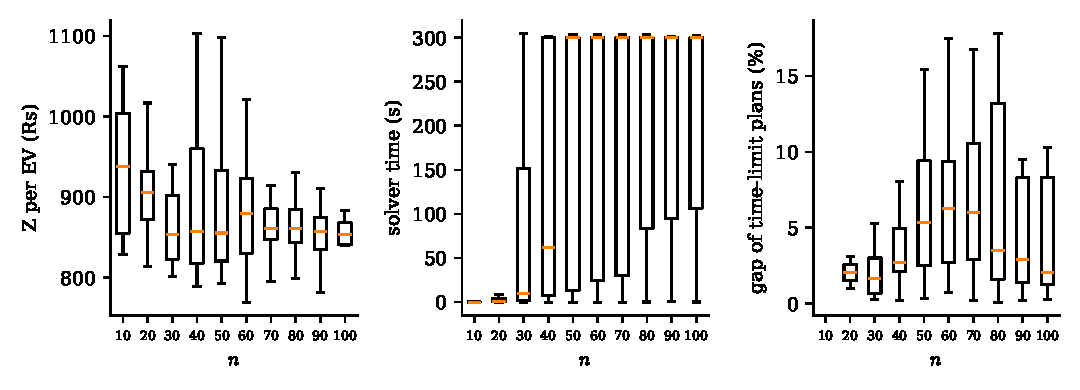
\includegraphics[width=\textwidth]{figures/inst_by_n.pdf}
\caption{Objective per EV, solver time and gap by instance size (boxes: middle 50\pct, line: median).}
\label{fig:instn}
\end{figure}
\begin{itemize}
  \item The objective per EV is fairly stable: \ZperMean{} Rs on average, between \ZperMin{} and \ZperMax{} Rs. It falls slightly with $n$ because the fixed van dispatch cost is shared by more EVs.
  \item About \VansMean{} vans leave per instance and serve about a fifth of the EVs (\VanPctMean\pct{} on average); most of them are the stranded EVs, who are \StrandedShare\pct{} of all EVs. Of the free-choice EVs only \FreeVanPctMean\pct{} get a van on average.
  \item Solver time reaches the \TimeLimit\,s limit from about $n=40$; the gaps of the time-limit plans are small (median \GapMed\pct).
\end{itemize}

\subsection{Families}
\begin{table}[H]
\centering\scriptsize
\caption{Results by Solomon family (means over valid plans; van shares over free-choice EVs).}
\label{tab:family}

\resizebox{\textwidth}{!}{\begin{tabular}{lrrrrrrrrrrr}\toprule
family & instances & \shortstack{valid\\plans} & \shortstack{Z per EV\\(Rs)} & \shortstack{operator\\share (\%)} & \shortstack{commercial\\EVs (\%)} & \shortstack{van share\\personal (\%)} & \shortstack{van share\\commercial (\%)} & \shortstack{mean queue\\(min)} & \shortstack{request to\\charged (min)} & \shortstack{vans\\used} & $T$ (min) \\ \midrule
C1 & 90 & 89 & 868 & 31.6 & 72.9 & 21.5 & 0.9 & 0.54 & 59.5 & 2.18 & 1236 \\
C2 & 80 & 79 & 882 & 30.6 & 66.9 & 21.8 & 0.6 & 0.69 & 61.5 & 1.90 & 3390 \\
R1 & 120 & 75 & 878 & 33.7 & 70.7 & 11.8 & 0.2 & 1.37 & 59.8 & 2.33 & 230 \\
R2 & 110 & 110 & 817 & 32.0 & 71.3 & 18.9 & 1.3 & 1.21 & 58.9 & 2.09 & 1000 \\
RC1 & 80 & 42 & 1036 & 29.7 & 56.4 & 18.2 & 0.5 & 1.55 & 74.6 & 2.43 & 240 \\
RC2 & 80 & 79 & 931 & 32.2 & 74.8 & 25.8 & 0.3 & 0.62 & 67.9 & 2.39 & 960 \\
\bottomrule\end{tabular}
}
\end{table}
\begin{figure}[H]
\centering
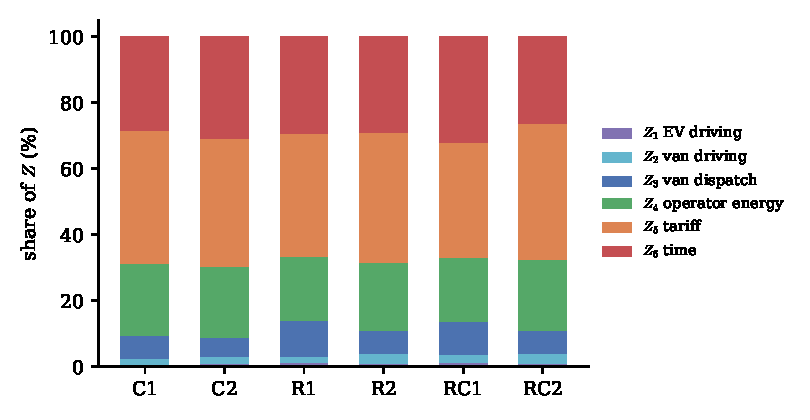
\includegraphics[width=0.72\textwidth]{figures/obj_family.pdf}
\caption{Composition of the objective by family.}
\label{fig:objfamily}
\end{figure}
The short-horizon families R1 and RC1 have the fewest valid plans (\ValidROne{} of \InstROne{} and \ValidRCOne{} of \InstRCOne): their horizon of 230--240 minutes leaves little room. RC1 is the dearest family per EV (\ZperRCOneMean{} Rs against \ZperRTwoMean{} Rs in R2). The composition of $Z$ is almost the same in every family: \OpShareMin--\OpShareMax\pct{} operator cost, the rest perceived customer cost. In every family personal EVs get vans far more often than commercial EVs.

\inshort{Families differ mainly in how often a plan exists (short horizons) and in cost level; the cost structure and the segment pattern are the same everywhere.}

\subsection{The two segments}
\begin{table}[H]
\centering\scriptsize
\caption{The two segments over all EVs of the \NValid{} valid plans (van share over free-choice EVs; queue over station users; van wait over van users).}
\label{tab:segments}

\resizebox{\textwidth}{!}{\begin{tabular}{lrrrrrrrrrrr}\toprule
segment & EVs & \shortstack{share\\(\%)} & \shortstack{stranded\\(\%)} & \shortstack{mean\\$\theta$} & \shortstack{free-choice\\by van (\%)} & \shortstack{mean FCS\\queue (min)} & \shortstack{FCS users\\queueing (\%)} & \shortstack{mean van\\wait (min)} & \shortstack{downtime\\(min)} & \shortstack{paid\\(Rs)} & \shortstack{perceived\\cost (Rs)} \\ \midrule
personal & 7043 & 29.6 & 13.5 & 0.69 & 19.9 & 0.41 & 2.8 & 19.8 & 60.6 & 352 & 662 \\
commercial & 16787 & 70.4 & 15.9 & 0.36 & 0.7 & 1.58 & 9.4 & 24.5 & 64.3 & 335 & 582 \\
\bottomrule\end{tabular}
}
\end{table}
\begin{itemize}
  \item Commercial EVs are \CommShareAll\pct{} of the \NEVsValid{} EVs, but only \CommShareOfFreeVan\pct{} of the free-choice EVs that get a van: \NFreeVanPersonal{} of the \NFreeVanPersonal{}+\NFreeVanCommercial{} free-choice van users are personal.
  \item Commercial drivers queue more at stations (\QueueCommercial{} against \QueuePersonal{} min on average) and are out of service longer (\DowntimeCommercial{} against \DowntimePersonal{} min from request to full charge).
  \item They pay about the same (\PayCommercial{} against \PayPersonal{} Rs) but feel less of it in total (\PercCommercial{} against \PercPersonal{} Rs perceived) because their minutes are priced at the downtime rate, below a rich personal driver's value of time.
\end{itemize}

\inshort{The segments are served differently: personal cars get the vans, commercial cars use the stations and absorb the queues.}

\subsection{EV-level distributions}
\begin{table}[H]
\centering\footnotesize
\caption{Distribution of EV-level variables (all EVs of valid plans unless stated).}
\label{tab:evstats}
\begin{tabular}{lrrrrrr}\toprule
variable (per EV) & count & mean & median & 10th pct & 90th pct & max \\ \midrule
income $\theta$ & 23830 & 0.46 & 0.42 & 0.18 & 0.83 & 1.00 \\
energy demand $E_i$ (kWh) & 23830 & 19.6 & 18.6 & 14.3 & 27.8 & 40.0 \\
nearest reachable FCS (km) & 20220 & 1.61 & 1.50 & 0.65 & 2.70 & 4.71 \\
demand pressure & 20220 & 0.46 & 0.21 & 0.03 & 1.38 & 2.59 \\
drive to FCS (km), FCS users & 18903 & 2.24 & 1.66 & 0.67 & 4.34 & 22.65 \\
FCS queue (min), FCS users & 18903 & 1.28 & 0.00 & 0.00 & 0.00 & 46.50 \\
van wait (min), van users & 4927 & 22.5 & 0.0 & 0.0 & 78.3 & 328.9 \\
charging time (min) & 23830 & 50.7 & 43.3 & 31.0 & 75.7 & 109.1 \\
request to charged (min) & 23830 & 63.2 & 59.4 & 38.7 & 95.3 & 380.5 \\
money paid (Rs) & 23830 & 340 & 327 & 234 & 511 & 1000 \\
perceived money (Rs) & 23830 & 352 & 322 & 200 & 530 & 1238 \\
perceived time (Rs) & 23830 & 253 & 204 & 115 & 459 & 1500 \\
perceived total (Rs) & 23830 & 605 & 570 & 404 & 881 & 2011 \\
\bottomrule\end{tabular}

\end{table}
\begin{figure}[H]
\centering
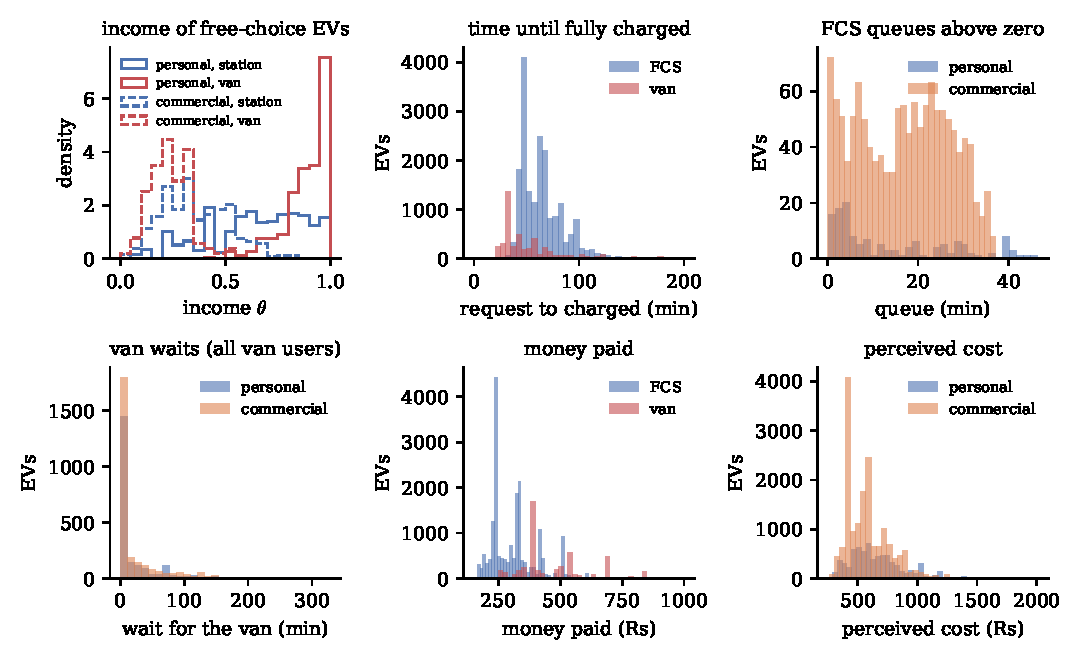
\includegraphics[width=\textwidth]{figures/ev_dists.pdf}
\caption{Distributions of income (by segment and resource), time until charged, queues, van waits, money paid and perceived cost.}
\label{fig:evdists}
\end{figure}
\begin{itemize}
  \item Personal van users are the richest group (top left): their mean income is \MeanThetaVanPers{} against \MeanThetaFCSPers{} for personal station users. Commercial incomes are lower and the few commercial van users are spread over low incomes.
  \item Most EVs are fully charged within about \TTCTen--\TTCNinety{} minutes of their request (10th to 90th percentile).
  \item Only \NQueued{} of the \NFCSfree{} free-choice station users queue at all; their queues spread up to about \QueueMax{} minutes, and most of them are commercial.
  \item \VanWaitZeroShare\pct{} of van users are served with no wait, but there is a long tail; Section~\ref{sec:choice} shows that the long waits belong to plans that were not proven optimal.
\end{itemize}

\subsection{Correlations}
\begin{figure}[H]
\centering
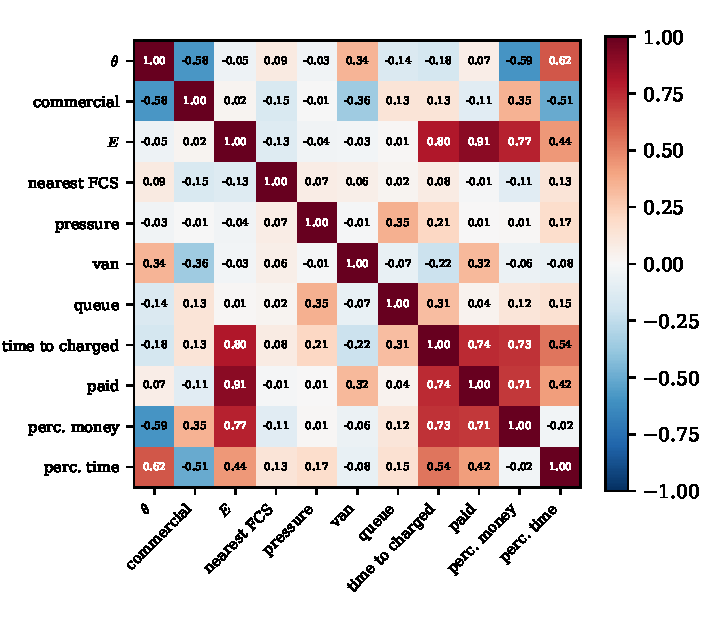
\includegraphics[width=0.6\textwidth]{figures/corr.pdf}
\caption{Spearman correlations between EV-level variables (free-choice EVs).}
\label{fig:corr}
\end{figure}
Income goes with being served by a van ($\rho=\CorrThetaVan$), being commercial against it ($\rho=\CorrCommVan$); the two are entangled because commercial drivers are poorer ($\rho=\CorrThetaComm$). Within the personal segment alone the correlation of income and van is $\rho=\CorrPersVanWithin$. Demand pressure is the strongest correlate of queueing ($\rho=\CorrPressQueue$), followed by being commercial ($\rho=\CorrCommQueue$). Income lowers the perceived money ($\rho=\CorrThetaPercMoney$) and raises the perceived time ($\rho=\CorrThetaPercTime$); money paid follows the energy demand ($\rho=\CorrEPay$).

\inshort{Income and segment together decide who gets a van; demand pressure and the commercial segment go with queues; energy goes with money paid.}

%=====================================================================
\clearpage
\part{Comprehensive analysis}
\section{Analysis point by point}

%---------------------------------------------------------------------
\subsection{Anatomy of the objective function}
\label{sec:anatomy}

\subsubsection{The six terms}
\[
Z=\underbrace{Z_1}_{\substack{\text{EV driving}\\\mu_i c^{\mathrm{EV}} d_{if}}}+\underbrace{Z_2}_{\substack{\text{van driving}\\ c^{\mathrm M}\,\text{km}}}+\underbrace{Z_3}_{\substack{\text{dispatch}\\ c^{\mathrm F}_m u_m}}+\underbrace{Z_4}_{\substack{\text{energy}\\ \pi^{\mathrm F}E_i,\ \pi^{\mathrm M}E_i/\eta}}+\underbrace{Z_5}_{\substack{\text{tariff}\\ \mu_i p E_i}}+\underbrace{Z_6}_{\substack{\text{time}\\ c^{a}_i\times\text{minutes}}}
\]
$Z_2+Z_3+Z_4$ is the operator's cost (\ZOperator\pct{} of $Z$ over all valid plans) and $Z_1+Z_5+Z_6$ the customers' perceived cost (\ZCustomer\pct). The largest single terms are the perceived tariff $Z_5$ (\ZFive\pct) and perceived time $Z_6$ (\ZSix\pct), then operator energy $Z_4$ (\ZFour\pct), van dispatch $Z_3$ (\ZThree\pct), van driving $Z_2$ (\ZTwo\pct) and EV driving $Z_1$ (\ZOne\pct). Commercial customers carry \CustShareComm\pct{} of the perceived cost. Time is \TimeShareCustPers\pct{} of what a personal customer feels but only \TimeShareCustComm\pct{} for a commercial one: low-income drivers feel money more than minutes.

\subsubsection{How sensitive is $Z$ to each coefficient? (envelope theorem)}
Every term of $Z$ is a coefficient times a quantity of the plan (km, kWh, minutes, vans). Write the optimal objective as $Z^{*}(c)=\min_{x}\sum_k c_k\,g_k(x)$. The \emph{envelope theorem} says that, as long as the optimal plan $x^{*}$ does not change,
\[
\frac{\partial Z^{*}}{\partial c_k}=g_k(x^{*}),\qquad
\text{elasticity}_k=\frac{c_k}{Z^{*}}\frac{\partial Z^{*}}{\partial c_k}=\frac{c_k\,g_k(x^{*})}{Z^{*}}=\text{share of }Z\text{ carried by }c_k .
\]
For a customer line $c(\theta)=c^{0}(1-\theta)+c^{1}\theta$ the quantities are $g_{c^{0}}=\sum_i(1-\theta_i)\,m_i$ and $g_{c^{1}}=\sum_i\theta_i\,m_i$ over the EVs of that segment, with $m_i$ the minutes (or the money paid, for $\mu$). Summing $c_k g_k$ over all coefficients rebuilds $Z$ of every plan to within \ZRecMax{} Rs (rounding of the stored minutes), so the table is complete. Because $Z^{*}(c)$ is a minimum of linear functions of $c$, it is \emph{concave}: after re-optimising, the true $Z^{*}$ is never above the linear prediction. The table is therefore an upper bound on how much $Z$ can rise.

\begin{table}[H]
\centering\scriptsize
\caption{Derivative and elasticity of $Z$ with respect to every coefficient (all valid plans). Superscripts of the customer lines: activity (D, Q, C, V), segment (P, C) and end point ($\theta=0$ or 1); for commercial EVs D, C and V are the downtime rate $\omega$.}
\label{tab:elasticity}
\begin{tabular}{llp{5.2cm}rrr}\toprule
coefficient & value & meaning & \shortstack{$\partial Z/\partial$coef.\\per plan} & \shortstack{elasticity\\(\%)} & \shortstack{Rs per plan\\for $+10\%$} \\ \midrule
$c^{\mathrm{EV}}$ & 4 & EV driving cost (Rs/km) & 96.9 & 0.88 & 39 \\
$c^{\mathrm{M}}$ & 15 & van driving cost (Rs/km) & 71.1 & 2.42 & 107 \\
$c^{\mathrm{F}}_m$ & 1500 & van dispatch cost (Rs) & 2.2 & 7.48 & 329 \\
$\pi^{\mathrm{F}}$ & 8.7 & grid energy at FCS (Rs/kWh) & 792.1 & 15.66 & 689 \\
$\pi^{\mathrm{M}}$ & 10.7 & van battery energy (Rs/kWh) & 216.1 & 5.26 & 231 \\
$p^{\mathrm{F}}$ & 15 & FCS tariff (Rs/kWh) & 847.1 & 28.88 & 1271 \\
$p^{\mathrm{M}}$ & 25 & van tariff (Rs/kWh) & 184.2 & 10.46 & 460 \\
$\mu^{P,0}$ & 1.5 & money sensitivity, personal, $\theta=0$ & 1558.7 & 5.31 & 234 \\
$\mu^{P,1}$ & 0.5 & money sensitivity, personal, $\theta=1$ & 3671.5 & 4.17 & 184 \\
$c^{\mathrm{D},P,0}$ & 1.5 & value of time D, personal, $\theta=0$ & 30.0 & 0.10 & 5 \\
$c^{\mathrm{D},P,1}$ & 15 & value of time D, personal, $\theta=1$ & 50.4 & 1.72 & 76 \\
$c^{\mathrm{Q},P,0}$ & 2.5 & value of time Q, personal, $\theta=0$ & 2.5 & 0.01 & 1 \\
$c^{\mathrm{Q},P,1}$ & 25 & value of time Q, personal, $\theta=1$ & 1.7 & 0.10 & 4 \\
$c^{\mathrm{C},P,0}$ & 1 & value of time C, personal, $\theta=0$ & 197.3 & 0.45 & 20 \\
$c^{\mathrm{C},P,1}$ & 10 & value of time C, personal, $\theta=1$ & 362.0 & 8.23 & 362 \\
$c^{\mathrm{V},P,0}$ & 0.5 & value of time V, personal, $\theta=0$ & 63.2 & 0.07 & 3 \\
$c^{\mathrm{V},P,1}$ & 5 & value of time V, personal, $\theta=1$ & 192.9 & 2.19 & 96 \\
$\mu^{C,0}$ & 1.5 & money sensitivity, commercial, $\theta=0$ & 7588.6 & 25.87 & 1138 \\
$\mu^{C,1}$ & 0.5 & money sensitivity, commercial, $\theta=1$ & 4282.5 & 4.87 & 214 \\
$c^{\mathrm{D},C,0}$ & 1.5 & value of time D, commercial, $\theta=0$ & 171.0 & 0.58 & 26 \\
$c^{\mathrm{D},C,1}$ & 6 & value of time D, commercial, $\theta=1$ & 92.1 & 1.26 & 55 \\
$c^{\mathrm{Q},C,0}$ & 2 & value of time Q, commercial, $\theta=0$ & 33.0 & 0.15 & 7 \\
$c^{\mathrm{Q},C,1}$ & 7.5 & value of time Q, commercial, $\theta=1$ & 13.7 & 0.23 & 10 \\
$c^{\mathrm{C},C,0}$ & 1.5 & value of time C, commercial, $\theta=0$ & 1032.9 & 3.52 & 155 \\
$c^{\mathrm{C},C,1}$ & 6 & value of time C, commercial, $\theta=1$ & 568.1 & 7.75 & 341 \\
$c^{\mathrm{V},C,0}$ & 1.5 & value of time V, commercial, $\theta=0$ & 235.0 & 0.80 & 35 \\
$c^{\mathrm{V},C,1}$ & 6 & value of time V, commercial, $\theta=1$ & 131.3 & 1.79 & 79 \\
\bottomrule\end{tabular}

\end{table}
\begin{figure}[H]
\centering
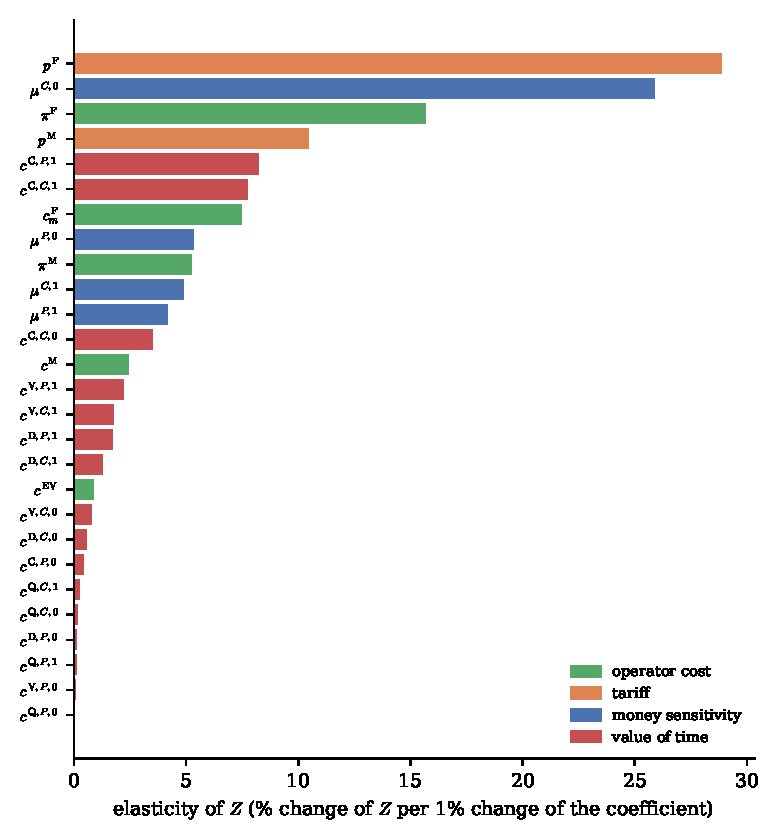
\includegraphics[width=0.6\textwidth]{figures/elasticity.pdf}
\caption{Elasticity of $Z$ with respect to each coefficient.}
\label{fig:elasticity}
\end{figure}
\begin{itemize}
  \item The most influential coefficients are \ElTopOneSym{} (elasticity \ElTopOne\pct), \ElTopTwoSym{} (\ElTopTwo\pct), \ElTopThreeSym{} (\ElTopThree\pct) and \ElTopFourSym{} (\ElTopFour\pct). A 10\pct{} rise of $p^{\mathrm F}$ would raise $Z$ by at most about \ElPFTen\pct.
  \item The money sensitivity of low-income commercial drivers is the single most influential customer number: commercial money sensitivities together carry \ElMoneyComm\pct{} of $Z$, personal ones \ElMoneyPers\pct. This is the segment mix at work: commercial drivers are the majority and mostly poor.
  \item Groups add up: operator coefficients $c^{\mathrm M},c^{\mathrm F},\pi^{\mathrm F},\pi^{\mathrm M}$ together \ElOperator\pct; all money sensitivities together \ElMoney\pct, the same as the tariffs and the EV driving cost together (\ElTariffs\pct), because the money terms are products $\mu\times p$; all value-of-time end points together \ElTime\pct{} (personal \ElTimePers\pct, commercial \ElTimeComm\pct).
  \item Queueing coefficients matter little in total (\ElQueueAll\pct{} for all four end points) because few EVs queue; they matter a lot \emph{locally}, for who queues (Section~\ref{sec:queues}).
  \item The dispatch cost $c^{\mathrm F}$ has a small total elasticity (\ElCF\pct) but a large effect on decisions: it decides when a van leaves at all (Section~\ref{sec:threshold}).
\end{itemize}

\inshort{About 70\pct{} of $Z$ is what customers feel and 30\pct{} what the operator pays. The station tariff, the money sensitivity of low-income commercial drivers and the grid price move $Z$ most; these elasticities are upper bounds because the plan can adapt.}

%---------------------------------------------------------------------
\subsection{Duality and shadow prices}
\label{sec:duals}

\subsubsection{Recap: duality in linear programming}
For a linear program in minimisation form
\[
\text{(P)}\quad \min\ c^{\top}x\ \ \text{s.t. } Ax\ge b,\ x\ge0
\qquad\Longleftrightarrow\qquad
\text{(D)}\quad \max\ b^{\top}y\ \ \text{s.t. } A^{\top}y\le c,\ y\ge0 ,
\]
strong duality gives equal optima, and the optimal dual value $y_k$ of constraint $k$ is its \emph{shadow price}: $y_k=\partial z^{*}/\partial b_k$, the change of the optimal cost when the right-hand side $b_k$ grows by one unit. \emph{Complementary slackness} says that a constraint with slack has $y_k=0$, and only binding constraints can have a non-zero price. The economic reading: $y_k$ is what one more unit of the resource behind constraint $k$ is worth.

\subsubsection{Why a MILP has no duals, and what we do instead}
In a MILP the 0/1 variables make the feasible set non-convex, so there is no dual in the LP sense, and the duals of the LP relaxation describe a fractional problem with weak big-$M$ constraints, not our plans. The standard remedy is the \emph{fixed-plan LP}: keep every yes/no decision of the plan (resource of each EV, order on each gun, every van route) and re-solve only the continuous part, the start times $S_i$ and the waits $q^{\mathrm F}_i$, $q^{\mathrm M}_i$:
\begin{align*}
\min\ & \textstyle\sum_{i\in\text{FCS}} c^{\mathrm Q}_i q^{\mathrm F}_i+\sum_{i\in\text{van}} c^{\mathrm V}_i q^{\mathrm M}_i\\
\text{FCS user } i:\ & S_i\ge r_i+t_{if},\quad q^{\mathrm F}_i=S_i-r_i-t_{if},\quad q^{\mathrm F}_i\le W_i,\quad S_i\le T-\tau^{\mathrm F}_i\\
i\text{ then }j\text{ on a gun}:\ & S_j\ge S_i+\tau^{\mathrm F}_i\\
\text{van user } i:\ & S_i\ge r_i,\quad q^{\mathrm M}_i=S_i-r_i,\quad S_i\le T-\tau^{\mathrm M}_i\\
\text{van route } 0\to a\to\dots\to b\to0:\ & S_a\ge t_{0a},\quad S_j\ge S_i+\tau^{\mathrm M}_i+t_{ij},\quad S_b\le T-\tau^{\mathrm M}_b-t_{b0}.
\end{align*}
For a commercial EV $c^{\mathrm Q}_i=\omega_i+\delta_i$ and $c^{\mathrm V}_i=\omega_i$. Everything else in $Z$ is constant once the decisions are fixed. The duals of this LP are the shadow prices \emph{of the plan}. We solved it with Gurobi for all \NLPPlans{} valid plans. \textbf{Check:} in every plan the LP optimum equals the plan's own waiting cost to within \LPDiffMax{} Rs (median \LPDiffMedian{} Rs; rounding of the stored times), so the LP reproduces the plans.

\begin{table}[H]
\centering\scriptsize
\caption{Shadow prices of the fixed-plan LPs, all valid plans (absolute values; mean, median and max over the non-zero duals).}
\label{tab:duals}
\begin{tabular}{p{3.6cm}rrrrrp{4.4cm}}\toprule
constraint & rows & \shortstack{non-zero\\dual (\%)} & \shortstack{mean\\(Rs/min)} & \shortstack{median\\(Rs/min)} & \shortstack{max\\(Rs/min)} & meaning of the dual \\ \midrule
FCS arrival $S_i\ge r_i+t_{if}$ & 18903 & 7.6 & 5.00 & 3.83 & 40.06 & not unique (degenerate); not interpreted \\
van release $S_i\ge r_i$ & 4927 & 54.0 & 4.26 & 3.88 & 17.72 & not unique (degenerate); not interpreted \\
gun order $S_j\ge S_i+\tau^{\mathrm{F}}_i$ & 10829 & 13.5 & 5.14 & 3.83 & 40.06 & value of one gun-minute: delay EV $i$ passes to those behind it \\
van order $S_j\ge S_i+\tau^{\mathrm{M}}_i+t_{ij}$ & 3887 & 38.7 & 5.51 & 4.28 & 19.02 & value of one van-minute on that leg \\
first stop $S_a\ge t_{0a}$ & 1040 & 72.6 & 8.31 & 7.73 & 22.97 & value of an earlier van departure \\
queue limit $q^{\mathrm{F}}_i\le W_i$ & 18903 & 0.0 & 0.00 & 0.00 & 0.00 & value of one more minute of patience \\
deadline $C_i\le T$, van return & 24870 & 0.0 & 0.00 & 0.00 & 0.00 & value of one more minute of horizon \\
\bottomrule\end{tabular}

\end{table}

\subsubsection{Gun-minutes: the price of congestion}
The dual of a gun-order constraint $S_j\ge S_i+\tau^{\mathrm F}_i$ is the value of one gun-minute at that moment: if EV $i$ held the gun one minute less, EV $j$ and everyone queued behind $j$ would start one minute earlier, and $Z$ would fall by the sum of their queueing rates $c^{\mathrm Q}$. It is the \emph{congestion externality} that EV $i$ imposes on the EVs behind it.
\begin{figure}[H]
\centering
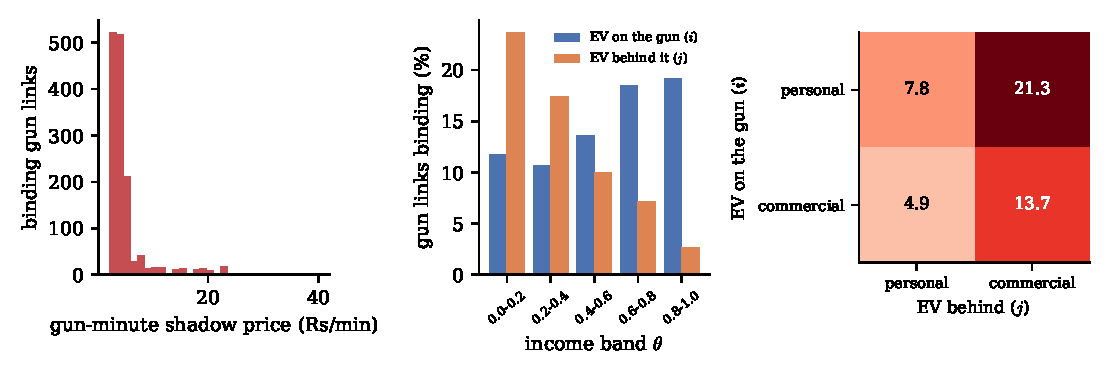
\includegraphics[width=\textwidth]{figures/gun_duals.pdf}
\caption{Left: gun-minute shadow prices where they are non-zero. Middle: share of binding gun links by income of the EV on the gun and of the EV behind it. Right: share binding (\%) by the segment of both.}
\label{fig:gunduals}
\end{figure}
\begin{table}[H]
\centering\small
\caption{Gun links by demand pressure of the EV behind.}
\label{tab:gunpressure}
\begin{tabular}{lrrrr}\toprule
\shortstack{demand pressure\\of the follower} & gun links & \shortstack{binding\\(\%)} & \shortstack{mean dual if\\binding (Rs/min)} & \shortstack{mean dual\\all links (Rs/min)} \\ \midrule
low & 6437 & 0.7 & 4.1 & 0.03 \\
medium & 2840 & 6.6 & 5.3 & 0.35 \\
high & 1552 & 78.8 & 5.2 & 4.06 \\
\bottomrule\end{tabular}

\end{table}
\begin{itemize}
  \item Of \NGunLinks{} consecutive gun links, \GunBindPct\pct{} are binding. Where binding, a gun-minute is worth \GunMean{} Rs on average (median \GunMedian, up to \GunMax{} Rs/min). This is lower than in formulation~3 because most EVs waiting behind are commercial drivers with a low queueing rate $c^{\mathrm Q,\mathrm C}$.
  \item Congestion is a peak phenomenon: \GunBindHigh\pct{} of gun links are binding when the EV behind arrives at high demand pressure, against \GunBindLow\pct{} at low pressure.
  \item \textbf{Who imposes the externality and who bears it.} By income: a link is binding in \GunBindRichOn\pct{} of the cases when the EV on the gun is in the richest band and \GunBindPoorOn\pct{} when it is in the poorest; seen from the EV behind it is the reverse: \GunBindPoorBehind\pct{} for the poorest and \GunBindRichBehind\pct{} for the richest. By segment (right panel): a link is binding most often when a personal EV holds the gun and a commercial EV waits (\GunBindPersOnCommBehind\pct{} of \GunNPersOnCommBehind{} links), least often in the opposite case (\GunBindCommOnPersBehind\pct).
  \item This is the queue priority of Section~\ref{sec:queues} in dual form: the model lets the customer with the higher queueing rate go first; the commercial or poorer EV waits because its $c^{\mathrm Q}$ is lower.
\end{itemize}

\subsubsection{Van-minutes}
The dual of a van-order constraint is the value of one van-minute on that leg: \VanBindPct\pct{} of van legs are binding, worth \VanDualMean{} Rs/min on average when binding. The EVs waiting for a van are mostly personal (driver-free rate $c^{\mathrm V,\mathrm P}$) or stranded.

\subsubsection{Patience limits and the deadline: zero shadow prices}
All \NPatience{} queue-limit constraints $q^{\mathrm F}_i\le W_i$ and all \NDeadline{} deadline and van-return constraints have shadow price zero in every plan, so $\partial Z/\partial T=0$ and $\partial Z/\partial W_i=0$ for every fixed plan. These constraints still matter, but only through the \emph{decisions}: they rule out plans (a queue longer than $W_i$, a van route too long for $T$), and the \NInf{} infeasible instances exist only because of the deadline. A fixed-plan LP cannot see that; measuring it needs re-solving the MILP with a longer $T$ or a larger $W$.

\subsubsection{The value of charger power}
The charging times depend on power: $\tau^{\mathrm F}_i=60E_i/P^{\mathrm F}$ and $\tau^{\mathrm M}_i=60E_i/P^{\mathrm M}$. By the chain rule, with the decisions fixed,
\[
\frac{\partial Z}{\partial P^{\mathrm F}}=\sum_{i\in\text{FCS}}\Big(c^{\mathrm C}_i+\lambda^{\text{gun}}_i-\lambda^{\text{deadline}}_i\Big)\frac{\partial\tau^{\mathrm F}_i}{\partial P^{\mathrm F}},\qquad \frac{\partial\tau^{\mathrm F}_i}{\partial P^{\mathrm F}}=-\frac{\tau^{\mathrm F}_i}{P^{\mathrm F}},
\]
where $c^{\mathrm C}_i$ is the customer's own charging-time rate ($\omega_i$ for a commercial EV) and $\lambda^{\text{gun}}_i$ the gun-minute price behind EV $i$.
\begin{figure}[H]
\centering
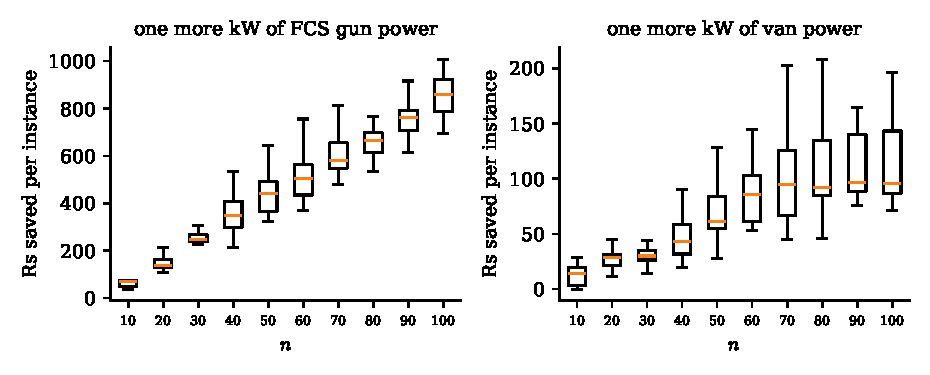
\includegraphics[width=0.78\textwidth]{figures/power_value.pdf}
\caption{Value of one more kW of charging power per instance, by instance size.}
\label{fig:power}
\end{figure}
One more kW of station-gun power (22 to 23\,kW) is worth \DPFmean{} Rs per instance on average (median \DPFmedian, up to \DPFmax), about \DPFperEV{} Rs per EV. \DPFcong\pct{} of it is congestion relief (shorter queues for the EVs behind), the rest is the customers' own shorter charging time. One more kW of van power is worth \DPMmean{} Rs per instance (up to \DPMmax). Faster station guns are worth about \DPFoverDPM{} times more than faster vans, because far more EVs charge at stations.

\subsubsection{What these shadow prices cannot tell}
\begin{itemize}
  \item They hold for the given decisions. Discrete resources (one more van, one more gun, one more seat $Q_m$, a larger battery) change the decisions and need re-solving the MILP; experiments E2 and E8 do that.
  \item The duals of the arrival and release constraints are not unique: when an EV starts the moment it arrives, both its arrival constraint and its zero-wait bound are binding (degenerate), and the solver may split the price between them. We report but do not interpret them.
\end{itemize}

\inshort{Fixing each plan's decisions gives an exact LP whose duals are the plan's shadow prices. Gun-minutes are the scarce resource at peak (\GunMean{} Rs/min when binding), and the price is paid mostly by commercial and poorer customers waiting behind richer personal ones. Patience limits and the deadline have zero marginal value; they act only by excluding plans. One more kW at the stations is worth about \DPFmean{} Rs per instance.}

%---------------------------------------------------------------------
\subsection{The income threshold of each segment: theory against data}
\label{sec:threshold}

\subsubsection{The formulas}
Section~``How segment and income enter the decision'' of the formulation compares, for one EV with everything else fixed, the cost of a van with the cost of its station. With $\Pi_i=(p^{\mathrm M}-p^{\mathrm F})E_i-c^{\mathrm{EV}}d_{if}$ the extra money the van costs the customer and $\kappa_i=(\pi^{\mathrm M}/\eta-\pi^{\mathrm F})E_i+c^{\mathrm M}x_i$ ($+c^{\mathrm F}$ if the van would not leave otherwise) the operator's extra cost,
\begin{align*}
\Delta^{\mathrm P}_i(\theta)&=\mu^{\mathrm P}(\theta)\,\Pi_i+\kappa_i-\Big[c^{\mathrm D,\mathrm P}(\theta)\,t_{if}+c^{\mathrm Q,\mathrm P}(\theta)\,q^{\mathrm F}_i+c^{\mathrm C,\mathrm P}(\theta)\,\tau^{\mathrm F}_i-c^{\mathrm V,\mathrm P}(\theta)\big(q^{\mathrm M}_i+\tau^{\mathrm M}_i\big)\Big],\\
\Delta^{\mathrm C}_i(\theta)&=\mu^{\mathrm C}(\theta)\,\Pi_i+\kappa_i-\omega(\theta)\,D_i-\delta(\theta)\,q^{\mathrm F}_i,\qquad D_i=t_{if}+q^{\mathrm F}_i+\tau^{\mathrm F}_i-\big(q^{\mathrm M}_i+\tau^{\mathrm M}_i\big).
\end{align*}
The van is chosen when $\Delta_i<0$. $D_i$ is the downtime the van saves a taxi. With straight-line sensitivities both are linear in $\theta$, so each segment has at most one threshold $\theta^{*}$ with $\Delta(\theta^{*})=0$.

\subsubsection{The numbers for a typical EV}
Take $E=\TypE$\,kWh, \TypD\,km to the nearest station ($t=\TypT$\,min), no station queue, a \TypQM-minute van wait and a \TypX\,km van detour. Then $\tau^{\mathrm F}=\TypTauF$\,min, $\tau^{\mathrm M}=\TypTauM$\,min, $\Pi=\TypPi$ Rs and $\kappa=\TypKappa$ Rs.
\begin{itemize}
  \item \textbf{Personal:} $\Delta^{\mathrm P}(0)=\DeltaPZero$ Rs and $\Delta^{\mathrm P}(1)=\DeltaPOne$ Rs, so $\theta^{*}_{\mathrm P}=\ThetaStarP$ (the personal lines are those of formulation~3, so the threshold is the same).
  \item \textbf{Commercial:} the van saves only $D=\TypDsaved$ minutes of downtime (the drive and the faster charging, minus the van wait). $\Delta^{\mathrm C}(0)=\DeltaCZero$ Rs and $\Delta^{\mathrm C}(1)=\DeltaCOne$ Rs: the van is dearer at \emph{every} income, so there is no threshold in $[0,1]$. A taxi has no driver-free benefit to set against the van premium $\Pi$.
\end{itemize}
Queues change this, because every queue minute raises the van's value to a taxi at the full rate $\omega+\delta$. Table~\ref{tab:commqueue} gives the station queue that makes the van the better choice for the typical commercial EV.
\begin{table}[H]
\centering\small
\caption{Typical commercial EV: extra cost of the van at no queue, and the station queue at which the van becomes the better choice, by income.}
\label{tab:commqueue}
\begin{tabular}{lrrrr}\toprule
$\theta$ & \shortstack{$\Delta^{\mathrm{C}}$ at no queue\\(Rs)} & \shortstack{queue that makes\\the van better (min)} & \shortstack{queue tolerance\\$W^{\mathrm{C}}(\theta)$ (min)} & \shortstack{same, van\\without wait (min)} \\ \midrule
0.00 & 393 & 196.7 & 40.0 & 189.2 \\
0.25 & 332 & 98.3 & 33.8 & 90.5 \\
0.50 & 270 & 56.8 & 27.5 & 48.9 \\
0.75 & 208 & 34.0 & 21.2 & 26.0 \\
1.00 & 146 & 19.5 & 15.0 & 11.5 \\
\bottomrule\end{tabular}

\end{table}
\begin{figure}[H]
\centering
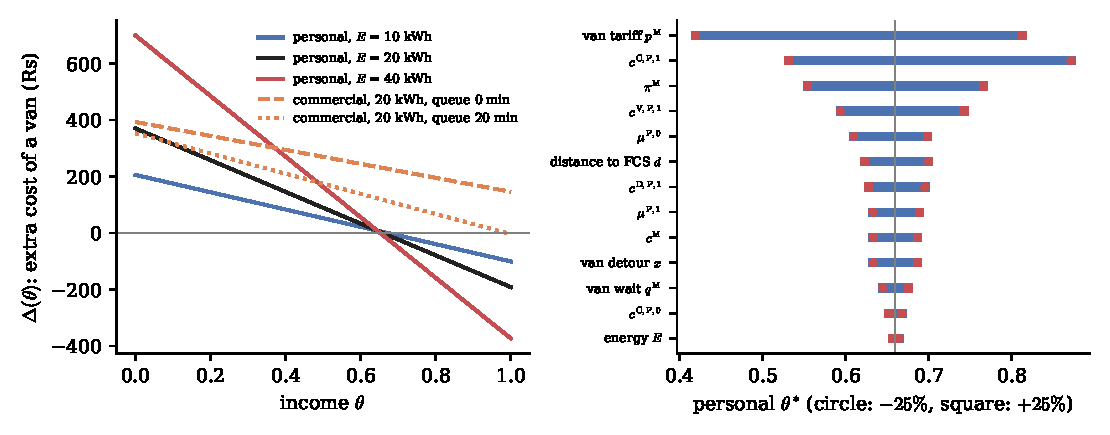
\includegraphics[width=\textwidth]{figures/threshold.pdf}
\caption{Left: extra cost of a van $\Delta(\theta)$ for personal EVs of three energy demands and for a commercial EV with no queue and a 20-minute queue. Right: how the personal $\theta^{*}$ moves when each parameter changes by $\pm25\%$.}
\label{fig:threshold}
\end{figure}
\begin{figure}[H]
\centering
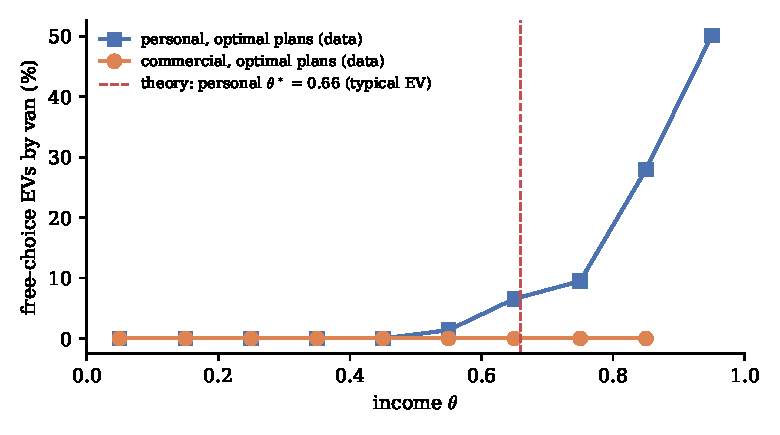
\includegraphics[width=0.7\textwidth]{figures/threshold_data.pdf}
\caption{Theory against data: van share of free-choice EVs in proven-optimal plans, by segment and income decile, and the predicted personal threshold.}
\label{fig:thresholddata}
\end{figure}
\begin{table}[H]
\centering\small
\caption{Personal threshold $\theta^{*}$ of the typical EV when one parameter changes by $\pm25\%$, sorted by swing.}
\label{tab:tornado}
\begin{tabular}{lrrrr}\toprule
parameter ($\pm25\%$) & $\theta^{*}$ at $-25\%$ & $\theta^{*}$ base & $\theta^{*}$ at $+25\%$ & swing \\ \midrule
van tariff $p^{\mathrm{M}}$ & 0.42 & 0.66 & 0.81 & 0.39 \\
$c^{\mathrm{C},\mathrm{P},1}$ & 0.87 & 0.66 & 0.53 & 0.34 \\
$\pi^{\mathrm{M}}$ & 0.55 & 0.66 & 0.77 & 0.21 \\
$c^{\mathrm{V},\mathrm{P},1}$ & 0.59 & 0.66 & 0.74 & 0.15 \\
$\mu^{\mathrm{P},0}$ & 0.61 & 0.66 & 0.70 & 0.09 \\
distance to FCS $d$ & 0.70 & 0.66 & 0.62 & 0.08 \\
$c^{\mathrm{D},\mathrm{P},1}$ & 0.70 & 0.66 & 0.63 & 0.07 \\
$\mu^{\mathrm{P},1}$ & 0.63 & 0.66 & 0.69 & 0.06 \\
$c^{\mathrm{M}}$ & 0.63 & 0.66 & 0.69 & 0.05 \\
van detour $x$ & 0.63 & 0.66 & 0.69 & 0.05 \\
van wait $q^{\mathrm{M}}$ & 0.64 & 0.66 & 0.68 & 0.03 \\
$c^{\mathrm{C},\mathrm{P},0}$ & 0.67 & 0.66 & 0.65 & 0.02 \\
energy $E$ & 0.66 & 0.66 & 0.66 & 0.01 \\
\bottomrule\end{tabular}

\end{table}

\subsubsection{What the thresholds explain}
\begin{itemize}
  \item \textbf{Personal: theory meets data.} In optimal plans no personal EV below $\theta=0.4$ gets a van (\VanPersBelowFour\pct); the share is \VanPersSixSeven\pct{} at 0.6--0.7, \VanPersEightNine\pct{} at 0.8--0.9 and \VanPersNineTen\pct{} at 0.9--1.0 (Figure~\ref{fig:thresholddata}). The predicted $\theta^{*}_{\mathrm P}=\ThetaStarP$ sits at the start of the rise.
  \item \textbf{Commercial: no threshold, as predicted.} In optimal plans the commercial van share is \VanCommOpt\pct{} in every decile. A commercial EV needs a station queue of \QNeededHalf{} minutes at $\theta=0.5$ and \QNeededOne{} minutes even at $\theta=1$ before the van pays off; at $\theta=1$ its queue tolerance is \WCommOne{} minutes, and at $\theta=0$ the queue needed (\QNeededZero{} min) is far above its tolerance of \WCommZero{} minutes. With a van that arrives at once, a rich taxi would switch at \QNeededOneNoWait{} minutes of queue.
  \item \textbf{Vans leave for the stranded, the rich personal owners fill the seats.} If the van must be sent out for a personal EV alone, $\Delta$ includes the dispatch cost $c^{\mathrm F}$ and stays positive at every income ($\Delta^{\mathrm P}(1)=\DeltaPOneDispatch$ Rs, $\theta^{*}=\ThetaStarPDispatch$). No free-choice customer ever justifies a van alone.
  \item \textbf{Queues lower the personal threshold, van waits raise it.} A 10-minute station queue lowers $\theta^{*}_{\mathrm P}$ to \ThetaStarPQten; a 40-minute van wait raises it to \ThetaStarPWaitForty. Distance matters ($\theta^{*}_{\mathrm P}=\ThetaStarPFar$ at 5\,km, \ThetaStarPNear{} at 0.5\,km), energy barely (\ThetaStarPEForty{} at 40\,kWh, \ThetaStarPETen{} at 10\,kWh).
  \item \textbf{Which parameters move the personal threshold most:} \TorTopSym{} (swing \TorTopSwing{} for $\pm25\%$), then the parameters of Table~\ref{tab:tornado}.
\end{itemize}

\inshort{For personal EVs the formulation predicts $\theta^{*}=\ThetaStarP$ and the optimal plans switch to vans there. For commercial EVs it predicts no threshold at all, because a taxi gains no driver-free time; only long station queues could justify a van, and the optimal plans give commercial free-choice EVs none.}

%---------------------------------------------------------------------
\subsection{Segment, income and the choice of resource}
\label{sec:choice}
\begin{figure}[H]
\centering
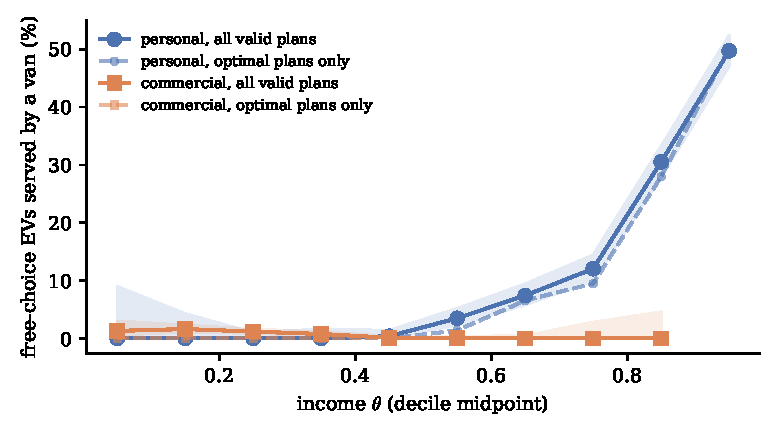
\includegraphics[width=0.7\textwidth]{figures/van_by_income.pdf}
\caption{Share of free-choice EVs served by a van, by segment and income decile (95\% Wilson interval shaded).}
\label{fig:vanincome}
\end{figure}
\begin{table}[H]
\centering\scriptsize
\caption{Van share by segment and income decile; 95\pct{} Wilson interval over all valid plans, and the share in proven-optimal plans.}
\label{tab:deciles}
\begin{tabular}{lrrrrrrrr}\toprule
 & \multicolumn{4}{c}{personal} & \multicolumn{4}{c}{commercial} \\
\cmidrule(lr){2-5}\cmidrule(lr){6-9} income $\theta$ & EVs & \shortstack{by van\\(\%)} & \shortstack{95\%\\interval} & \shortstack{optimal\\plans (\%)} & EVs & \shortstack{by van\\(\%)} & \shortstack{95\%\\interval} & \shortstack{optimal\\plans (\%)} \\ \midrule
0.0--0.1 & 39 & 0.0 & [0.0, 9.0] & 0.0 & 384 & 1.3 & [0.6, 3.0] & 0.0 \\
0.1--0.2 & 86 & 0.0 & [0.0, 4.3] & 0.0 & 1913 & 1.6 & [1.1, 2.3] & 0.0 \\
0.2--0.3 & 375 & 0.0 & [0.0, 1.0] & 0.0 & 3222 & 1.2 & [0.9, 1.6] & 0.0 \\
0.3--0.4 & 233 & 0.0 & [0.0, 1.6] & 0.0 & 3141 & 0.8 & [0.5, 1.1] & 0.0 \\
0.4--0.5 & 521 & 0.4 & [0.1, 1.4] & 0.0 & 2456 & 0.1 & [0.0, 0.4] & 0.0 \\
0.5--0.6 & 660 & 3.5 & [2.3, 5.2] & 1.4 & 1942 & 0.1 & [0.0, 0.4] & 0.0 \\
0.6--0.7 & 822 & 7.4 & [5.8, 9.4] & 6.6 & 854 & 0.0 & [0.0, 0.4] & 0.0 \\
0.7--0.8 & 846 & 12.1 & [10.0, 14.4] & 9.5 & 133 & 0.0 & [0.0, 2.8] & 0.0 \\
0.8--0.9 & 1166 & 30.5 & [28.0, 33.2] & 28.0 & 80 & 0.0 & [0.0, 4.6] & 0.0 \\
0.9--1.0 & 1347 & 49.7 & [47.1, 52.4] & 50.2 & 0 & -- & -- & -- \\
\bottomrule\end{tabular}

\end{table}
\begin{itemize}
  \item Overall \VanSharePersonal\pct{} of free-choice personal EVs and \VanShareCommercial\pct{} of free-choice commercial EVs get a van (\VanPersOpt\pct{} and \VanCommOpt\pct{} in optimal plans). Personal van users have a mean income of \MeanThetaVanPers{} against \MeanThetaFCSPers{} for personal station users.
  \item \textbf{The commercial van users are artefacts of unfinished optimisation.} All \NFreeVanCommercial{} free-choice commercial EVs served by a van come from time-limit plans (\CommVanTL\pct), \CommVanHighPressPct\pct{} of them at high demand pressure (mean pressure \CommVanPressure{} against \CommFCSPressure{} for commercial station users). They wait \CommVanWait{} min for the van on average, against \RichPersVanWait{} min for rich personal van users.
  \item The same holds for low incomes: the \NLowVan{} van users with $\theta<0.4$ are all commercial (\NLowVanComm) and none is in an optimal plan (\NLowVanOpt); they wait \LowVanWait{} min on average. They are not a property of the model.
\end{itemize}

\subsubsection{Logistic regression}
\begin{table}[H]
\centering\small
\caption{Logistic regression of $P(\text{served by a van})$ over the \LogitN{} free-choice EVs of all valid plans.}
\label{tab:logit}
\begin{tabular}{lrrrr}\toprule
term & coefficient & std. error & $z$ & $p$-value \\ \midrule
intercept & -8.401 & 0.343 & -24.5 & $<0.001$ \\
income $\theta$ & 9.166 & 0.331 & 27.7 & $<0.001$ \\
commercial & 1.883 & 0.791 & 2.4 & 0.017 \\
$\theta\times$ commercial & -15.387 & 0.922 & -16.7 & $<0.001$ \\
medium pressure & -0.612 & 0.088 & -6.9 & $<0.001$ \\
high pressure & -0.515 & 0.100 & -5.1 & $<0.001$ \\
commercial $\times$ high pressure & 5.543 & 0.721 & 7.7 & $<0.001$ \\
long horizon (type 2) & 0.016 & 0.077 & 0.2 & 0.834 \\
energy $E_i$ (per 10 kWh) & -0.211 & 0.062 & -3.4 & $<0.001$ \\
nearest reachable FCS (km) & 0.210 & 0.046 & 4.6 & $<0.001$ \\
\bottomrule\end{tabular}

\end{table}
Income has a strong positive effect for personal EVs: $+0.1$ in $\theta$ raises the probability of a van by \AMEThetaPers{} percentage points on average (average marginal effect). For commercial EVs the effect is \AMEThetaComm{} points: income does not buy a commercial EV a van. Distance to the nearest station raises the probability, energy demand lowers it, as the threshold formulas predict; the commercial--high-pressure interaction captures the few commercial van users of congested time-limit plans. The model classifies \LogitAcc\pct{} of EVs correctly (always predicting ``station'' would give \LogitBaseAcc\pct; McFadden pseudo-$R^2$ \LogitPseudoR).

\inshort{Segment first, income second: personal EVs get vans above a threshold near $\theta^{*}$, commercial EVs do not get vans in optimal plans whatever their income. Commercial and low-income van users exist only in unfinished plans.}

%---------------------------------------------------------------------
\subsection{Queues, priority and driving}
\label{sec:queues}
\begin{figure}[H]
\centering
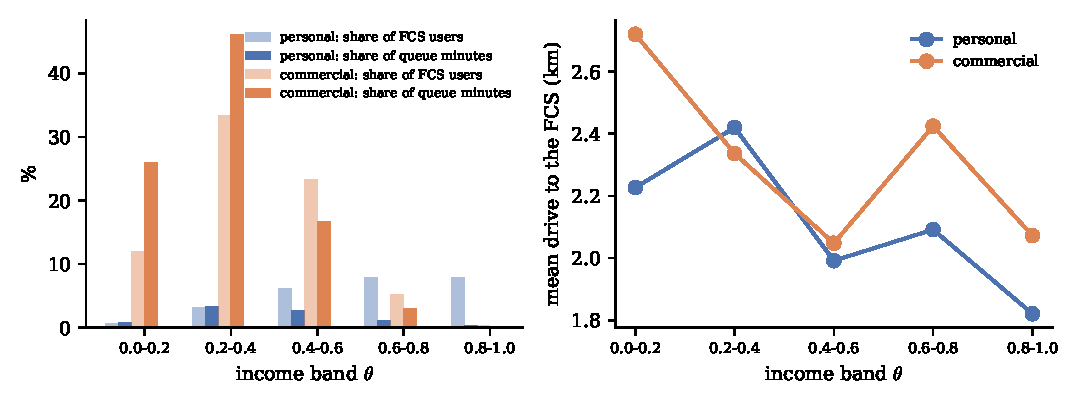
\includegraphics[width=\textwidth]{figures/queues_drive.pdf}
\caption{Left: share of station users and of all queue minutes by segment and income band. Right: mean distance driven to the station.}
\label{fig:queues}
\end{figure}
\begin{table}[H]
\centering\scriptsize
\caption{Free-choice station users by segment and income band.}
\label{tab:queues}
\begin{tabular}{lrrrrrrrrr}\toprule
segment & income $\theta$ & \shortstack{FCS\\users} & \shortstack{share of\\users (\%)} & \shortstack{share of queue\\minutes (\%)} & \shortstack{queueing\\(\%)} & \shortstack{mean queue\\(min)} & \shortstack{longest\\queue (min)} & \shortstack{largest\\$W_i$ (min)} & \shortstack{drive to\\FCS (km)} \\ \midrule
personal & 0.0--0.2 & 125 & 0.7 & 0.7 & 8.0 & 1.45 & 31.3 & 57.4 & 2.23 \\
 & 0.2--0.4 & 608 & 3.2 & 3.3 & 5.3 & 1.32 & 46.5 & 50.3 & 2.42 \\
 & 0.4--0.6 & 1156 & 6.1 & 2.7 & 3.3 & 0.57 & 40.4 & 42.0 & 1.99 \\
 & 0.6--0.8 & 1505 & 8.0 & 1.1 & 2.5 & 0.18 & 29.8 & 32.9 & 2.09 \\
 & 0.8--1.0 & 1487 & 7.9 & 0.4 & 1.5 & 0.06 & 12.7 & 24.0 & 1.82 \\
commercial & 0.0--0.2 & 2261 & 12.0 & 25.9 & 13.5 & 2.77 & 37.2 & 39.3 & 2.72 \\
 & 0.2--0.4 & 6301 & 33.3 & 46.0 & 10.4 & 1.76 & 33.8 & 35.0 & 2.34 \\
 & 0.4--0.6 & 4393 & 23.2 & 16.7 & 6.7 & 0.92 & 29.5 & 30.0 & 2.05 \\
 & 0.6--0.8 & 987 & 5.2 & 3.1 & 6.3 & 0.75 & 23.8 & 24.8 & 2.42 \\
 & 0.8--1.0 & 80 & 0.4 & 0.0 & 0.0 & 0.00 & 0.0 & 19.8 & 2.07 \\
\bottomrule\end{tabular}

\end{table}
\begin{itemize}
  \item Commercial drivers are \UserShareComm\pct{} of station users but do \QShareComm\pct{} of all queueing. The poorest 40\pct{} by income are \UserShareBottom\pct{} of users and do \QShareBottom\pct; the richest 20\pct{} are \UserShareTop\pct{} of users and do \QShareTop\pct.
  \item At the same income the commercial driver queues longer: for $\theta$ 0.2--0.6 the mean queue is \QueueMidComm{} min for commercial and \QueueMidPers{} min for personal EVs, because a personal driver's queueing rate is higher at equal income.
  \item Mechanism: when two EVs want the same gun, the one with the higher queueing rate $c^{\mathrm Q}$ goes first; the gun-minute shadow prices of Section~\ref{sec:duals} show the same pattern from the dual side.
  \item Every queue respects its tolerance $W_i$, and the queue-limit constraints carry no shadow price (Section~\ref{sec:duals}); still, the longest queue reaches \QueueMaxOverW\pct{} of its own $W_i$, and \NearLimit{} station users queue at more than 90\pct{} of theirs.
  \item Low-income users drive farther (\DriveBottom{} against \DriveTop{} km for the richest band; commercial \DriveComm{} against personal \DrivePers{} km): the free guns at the nearest stations go to customers whose time is worth more.
\end{itemize}

\inshort{Queue priority and the nearest free guns go to higher values of time: rich personal drivers first, commercial and poorer drivers wait and drive more. This is the cost-minimising plan under the formulation's values of time, and an equity issue the operator would have to decide on.}

%---------------------------------------------------------------------
\subsection{Peak and off-peak: demand pressure}
\label{sec:peak}
Demand pressure and its terciles are defined in Section~\ref{sec:defs} (low $\le\PressLow$, high $>\PressHigh$, pooled over all \NPressPoolInst{} baseline instances).
\begin{figure}[H]
\centering
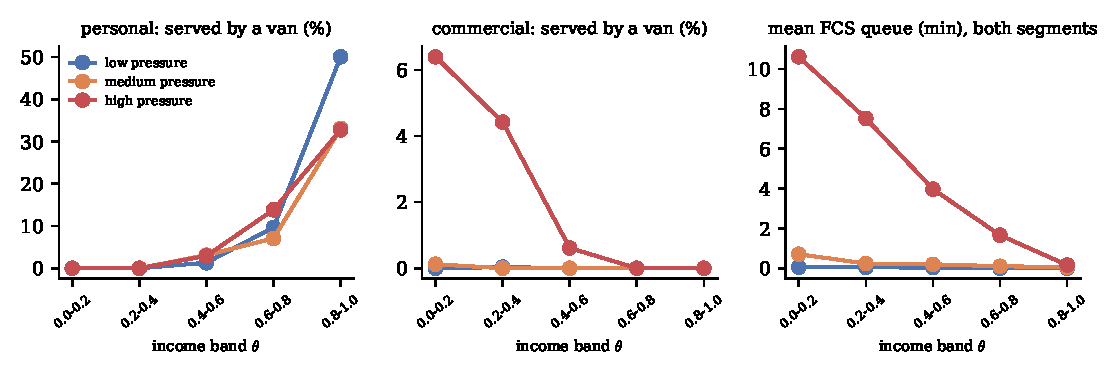
\includegraphics[width=\textwidth]{figures/pressure.pdf}
\caption{Van share by income band for low, medium and high demand pressure (personal, commercial) and mean station queue by income band.}
\label{fig:pressure}
\end{figure}
\begin{table}[H]
\centering\scriptsize
\caption{Free-choice EVs by demand pressure.}
\label{tab:pressure}
\begin{tabular}{lrrrrrrrr}\toprule
\shortstack{demand\\pressure} & EVs & \shortstack{queueing\\(\%)} & \shortstack{mean queue\\(min)} & \shortstack{by van (\%)\\personal} & \shortstack{by van (\%)\\commercial} & \shortstack{personal by van\\$\theta$ 0.0--0.2} & \shortstack{personal by van\\$\theta$ 0.4--0.6} & \shortstack{personal by van\\$\theta$ 0.8--1.0} \\ \midrule
low & 9480 & 0.5 & 0.03 & 23.4 & 0.0 & 0.0 & 1.3 & 50.0 \\
medium & 6378 & 3.1 & 0.26 & 17.1 & 0.0 & 0.0 & 3.1 & 33.1 \\
high & 4362 & 30.3 & 5.52 & 16.6 & 3.4 & 0.0 & 2.9 & 32.7 \\
\bottomrule\end{tabular}

\end{table}
\begin{itemize}
  \item Queues exist almost only at high pressure: \QueueLow, \QueueMedium{} and \QueueHigh{} min on average at low, medium and high pressure; \QueueingHigh\pct{} of station users queue at high pressure.
  \item At medium and high pressure fewer of the richest personal owners get a van (\VanRichPersLow\pct{} at low, \VanRichPersMedium\pct{} at medium, \VanRichPersHigh\pct{} at high pressure): the vans are already committed to stranded EVs.
  \item The formulation predicts that queues push commercial EVs towards vans; the data show a small rise only (\VanCommLow\pct, \VanCommMedium\pct, \VanCommHigh\pct), and only in time-limit plans (Section~\ref{sec:choice}).
  \item Instead, income and segment buy priority at the station: at high pressure poor commercial drivers ($\theta<0.4$) queue \QueuePoorCommHigh{} min on average, the richest personal owners \QueueRichPersHigh{} min.
\end{itemize}

\inshort{Peak demand creates the queues; at peak the vans are taken by stranded EVs, and segment and income buy a place at the station rather than a van.}

%---------------------------------------------------------------------
\subsection{Planning horizon and layout}
\label{sec:horizon}
\begin{figure}[H]
\centering
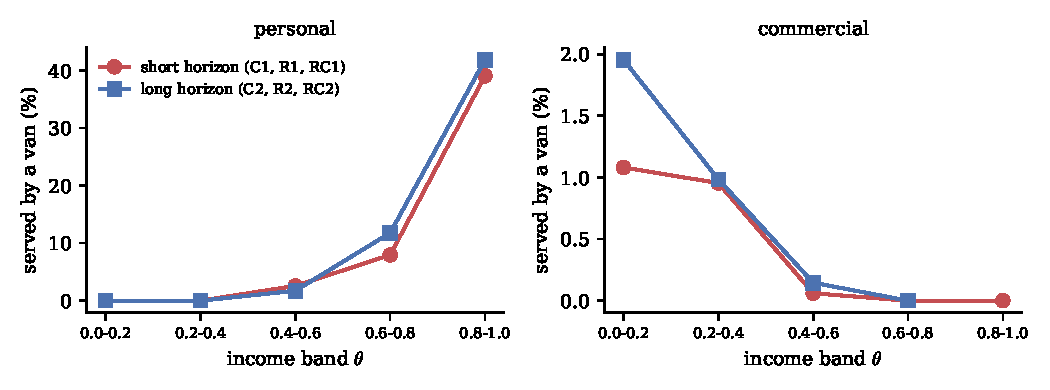
\includegraphics[width=0.85\textwidth]{figures/horizon.pdf}
\caption{Van share by income band, short-horizon against long-horizon families, per segment.}
\label{fig:horizon}
\end{figure}
\begin{table}[H]
\centering\scriptsize
\caption{Van share of free-choice EVs by family; personal EVs by income band.}
\label{tab:familyband}
\begin{tabular}{lrrrrrrrrrr}\toprule
family & horizon & EVs & \shortstack{mean\\pressure} & \shortstack{personal\\by van (\%)} & \shortstack{personal\\$\theta$ 0.0--0.2} & \shortstack{personal\\$\theta$ 0.2--0.4} & \shortstack{personal\\$\theta$ 0.4--0.6} & \shortstack{personal\\$\theta$ 0.6--0.8} & \shortstack{personal\\$\theta$ 0.8--1.0} & \shortstack{commercial\\by van (\%)} \\ \midrule
C1 & short & 4019 & 0.35 & 21.5 & 0.0 & -- & 0.0 & 2.0 & 47.3 & 0.9 \\
C2 & long & 3771 & 0.29 & 21.8 & 0.0 & 0.0 & 1.2 & 11.9 & 41.8 & 0.6 \\
R1 & short & 2415 & 0.67 & 11.8 & 0.0 & 0.0 & 7.7 & 8.8 & 25.0 & 0.2 \\
R2 & long & 5082 & 0.56 & 18.9 & -- & 0.0 & 2.4 & 10.4 & 36.8 & 1.3 \\
RC1 & short & 1338 & 0.64 & 18.2 & -- & 0.0 & 3.2 & 12.9 & 34.4 & 0.5 \\
RC2 & long & 3595 & 0.42 & 25.8 & 0.0 & 0.0 & 0.9 & 14.4 & 51.0 & 0.3 \\
\bottomrule\end{tabular}

\end{table}
Rich personal owners get a van slightly more often with a long horizon (\VanTopPersonalLong\pct{} against \VanTopPersonalShort\pct{} in the top band). Short horizons also mean higher demand pressure (\PressShort{} against \PressLong); with pressure in the regression, the horizon has little separate effect. Commercial EVs hardly get vans with either horizon.

\inshort{The horizon matters through congestion and through the vans' time budget (next section).}

%---------------------------------------------------------------------
\subsection{Infrastructure utilisation}
\label{sec:util}
How much of the installed infrastructure do the plans use? Definitions (\texttt{common/infra.py}, the same in the three reports), over the \NValid{} valid plans:
\begin{itemize}
  \item \textbf{Gun $g$:} busy minutes = sum of the station charging times $\tau^{\mathrm F}$ of its EVs; utilisation = busy minutes $/\,T$. Power is constant (22\,kW), so time utilisation equals energy utilisation (kWh delivered $/$ $22\,T/60$). A station is the mean of its two guns; the FCS system is total busy minutes $/(24\,T)$.
  \item \textbf{Active demand window} (data only): from the first request to the latest moment an EV could finish charging at a station if served at once, $[\min_i r_i,\ \max_i(r_i+\tau^{\mathrm F}_i)]$. Gun utilisation over this window is total busy minutes $/(24\times$ its length$)$; it removes the part of $[0,T]$ in which no demand can exist.
  \item \textbf{System:} energy delivered $/$ (installed power $\times\,T/60$), installed power $24\times22+5\times30=\UInstalledKW$\,kW (\UGunKWShare\pct{} of it at the stations).
\end{itemize}

\subsubsection{Stations and guns}
\begin{table}[H]
\centering\scriptsize
\caption{Utilisation by family (means over valid plans). ``Active window'': length of the data-only demand window as a share of $T$.}
\label{tab:utilfamily}
\resizebox{\textwidth}{!}{\begin{tabular}{lrrrrrrrrrr}\toprule
family & $T$ & plans & \shortstack{gun use\\over $[0,T]$ (\%)} & \shortstack{active window\\(\% of $T$)} & \shortstack{gun use over\\active window (\%)} & \shortstack{90th pct\\one gun (\%)} & \shortstack{idle guns\\(of 24)} & \shortstack{peak guns\\at once} & \shortstack{system\\use (\%)} & \shortstack{energy by\\van (\%)} \\ \midrule
C1 & 1236 & 89 & 8.0 & 76 & 10.4 & 21.8 & 9.4 & 11.3 & 7.9 & 20.8 \\
C2 & 3390 & 79 & 3.0 & 85 & 3.5 & 7.5 & 8.3 & 8.9 & 2.9 & 19.7 \\
R1 & 230 & 75 & 26.9 & 87 & 30.9 & 53.8 & 5.7 & 15.6 & 26.2 & 20.3 \\
R2 & 1000 & 110 & 9.2 & 78 & 11.7 & 19.8 & 4.9 & 14.4 & 8.8 & 18.8 \\
RC1 & 240 & 42 & 30.0 & 83 & 36.7 & 63.1 & 6.3 & 16.7 & 28.1 & 16.9 \\
RC2 & 960 & 79 & 10.7 & 78 & 13.9 & 22.8 & 7.4 & 12.0 & 10.4 & 20.4 \\
\bottomrule\end{tabular}
}
\end{table}
\begin{table}[H]
\centering\small
\caption{Utilisation by instance size (means over valid plans).}
\label{tab:utiln}
\resizebox{\textwidth}{!}{\begin{tabular}{lrrrrrrrr}\toprule
$n$ & plans & \shortstack{energy\\asked (kWh)} & \shortstack{gun use\\over $[0,T]$ (\%)} & \shortstack{gun use over\\active window (\%)} & \shortstack{idle guns\\(of 24)} & \shortstack{peak guns\\at once} & \shortstack{fleet use\\(\% of 5 vans)} & \shortstack{system\\use (\%)} \\ \midrule
10 & 55 & 191 & 3.5 & 4.6 & 18.5 & 3.7 & 18.2 & 3.4 \\
20 & 55 & 396 & 6.9 & 8.8 & 13.6 & 7.1 & 24.4 & 6.9 \\
30 & 55 & 589 & 11.0 & 13.7 & 9.5 & 11.0 & 28.0 & 10.3 \\
40 & 55 & 796 & 15.0 & 18.5 & 6.2 & 13.9 & 35.6 & 13.9 \\
50 & 53 & 981 & 17.1 & 20.7 & 4.8 & 15.3 & 46.0 & 16.5 \\
60 & 49 & 1178 & 18.2 & 21.7 & 4.1 & 15.9 & 55.9 & 17.7 \\
70 & 44 & 1364 & 17.4 & 20.4 & 2.4 & 16.7 & 57.7 & 17.0 \\
80 & 39 & 1560 & 14.8 & 18.2 & 1.6 & 16.4 & 63.6 & 14.5 \\
90 & 36 & 1773 & 12.8 & 15.9 & 1.0 & 16.9 & 68.9 & 12.5 \\
100 & 33 & 1964 & 14.5 & 18.1 & 0.3 & 17.5 & 69.1 & 14.0 \\
\bottomrule\end{tabular}
}
\end{table}
\begin{figure}[H]
\centering
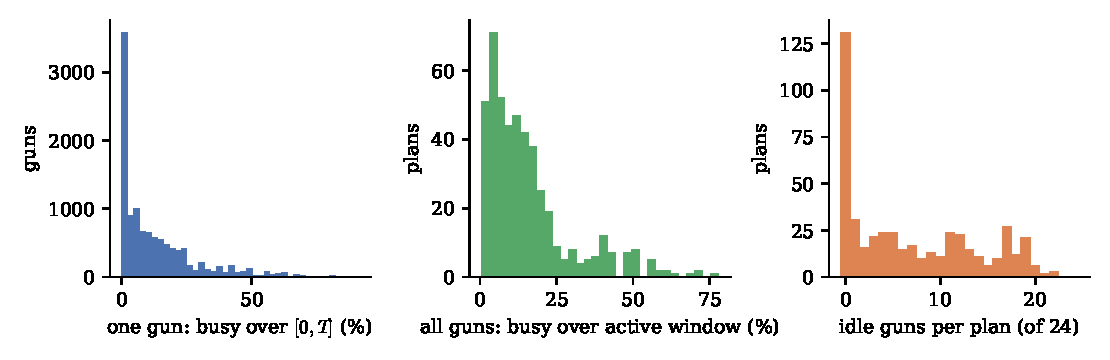
\includegraphics[width=\textwidth]{figures/util_guns.pdf}
\caption{Left: utilisation of every gun over $[0,T]$. Middle: utilisation of all guns over the active demand window, per plan. Right: guns without any EV, per plan.}
\label{fig:utilguns}
\end{figure}
\begin{figure}[H]
\centering
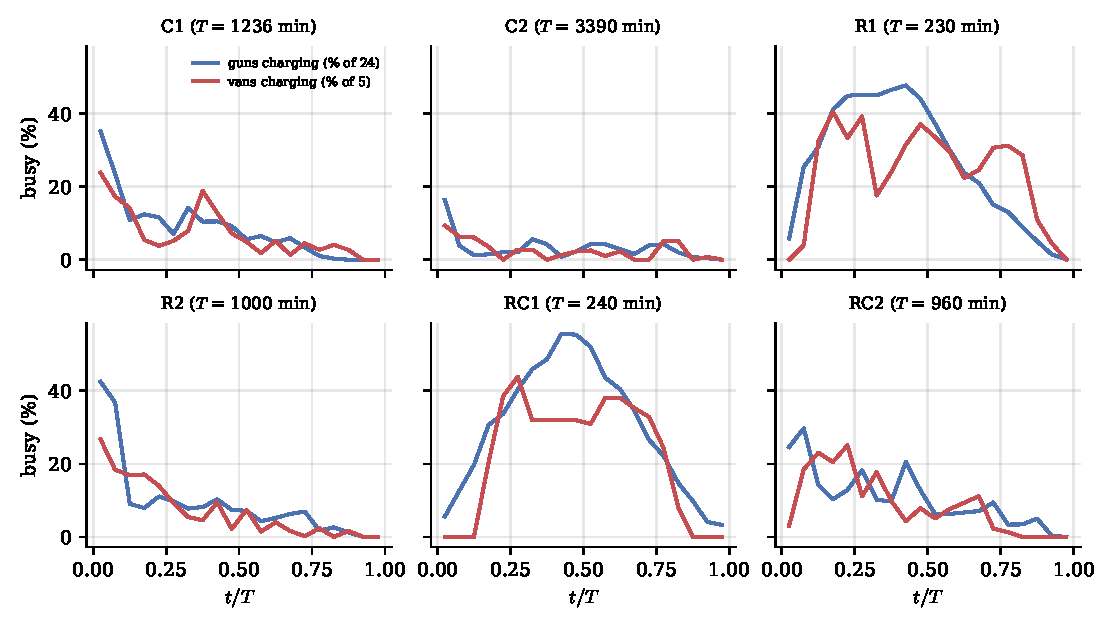
\includegraphics[width=0.9\textwidth]{figures/util_profile.pdf}
\caption{Busy profile: share of the 24 guns and of the 5 vans charging at time $t$ (20 bins of $t/T$, mean over the valid plans of each family).}
\label{fig:utilprofile}
\end{figure}
\begin{itemize}
  \item The guns are lightly used: over $[0,T]$ the FCS system is busy \UGunMean\pct{} of the time on average (median \UGunMedian\pct). A single gun is busy \UPerGunMean\pct{} of the time on average, \UPerGunNinety\pct{} at the 90th percentile and at most \UPerGunMax\pct; \UGunIdleShare\pct{} of all guns (\UStationIdleShare\pct{} of stations) charge no EV at all, \UIdleGunsMean{} of 24 per plan on average (\UIdleGunsTen{} at $n=10$, \UIdleGunsHundred{} at $n=100$).
  \item \textbf{The horizon decides the level.} Short horizons (C1, R1, RC1) use \UGunShort\pct{} of gun time, long horizons (C2, R2, RC2) \UGunLong\pct: the same 10--100 EVs are spread over periods of 230 to 3390 minutes.
  \item Requests span most of the period in every family (the active window is \UActiveShareShort\pct{} of $T$ for short and \UActiveShareLong\pct{} for long horizons), so restricting to it changes little: \UGunActiveShort\pct{} and \UGunActiveLong\pct{} (\UGunActiveMean\pct{} overall; \UGunActiveTen\pct{} at $n=10$ and \UGunActiveHundred\pct{} at $n=100$). Low utilisation over $[0,T]$ is not only empty time after the last request.
  \item \textbf{Where demand sits.} The busy profile of R1 and RC1 peaks at $t/T\approx\UProfilePeakBinShort$ with \UProfileMaxShort\pct{} of guns charging; that of C2, R2 and RC2 peaks right at the start ($t/T\approx\UProfilePeakBinLong$, \UProfileMaxLong\pct, the burst of requests at $t=0$ in Solomon's files) and falls to \UProfileLateLong\pct{} after $0.8\,T$.
  \item \textbf{Peak concurrency.} On average at most \UPeakGunsMean{} guns charge at the same moment (\UPeakGunsHundred{} at $n=100$); in \UPeakGunsFull{} plans all 24 guns are busy at once, and at most \UPeakVansMax{} vans charge at once.
\end{itemize}

\subsubsection{System and pressure}
\begin{table}[H]
\centering\small
\caption{Share of the 24 guns busy at the request time of free-choice EVs, by demand pressure tercile.}
\label{tab:utilpressure}
\begin{tabular}{lrrrr}\toprule
\shortstack{demand pressure\\of the EV} & free-choice EVs & \shortstack{guns busy at its\\request, mean (\%)} & \shortstack{90th\\pct (\%)} & \shortstack{half or more\\of guns busy (\%)} \\ \midrule
low & 9480 & 6.2 & 12.5 & 0.6 \\
medium & 6378 & 23.3 & 50.0 & 10.3 \\
high & 4362 & 21.8 & 87.5 & 26.0 \\
\bottomrule\end{tabular}

\end{table}
\begin{itemize}
  \item The valid plans charge \UEnergyTotal{} MWh in all, \UEnergyPerInst{} kWh per instance; \UEnergyFCSShare\pct{} at stations and \UEnergyVanShare\pct{} by vans.
  \item Of the installed power over $[0,T]$ the plans use \USystemMean\pct{} on average (at most \USystemMax\pct; \USystemShort\pct{} for short and \USystemLong\pct{} for long horizons).
  \item Pressure and busy guns: when a low-pressure EV requests, \UBusyAtRLow\pct{} of guns are charging on average; for medium and high pressure \UBusyAtRMedium\pct{} and \UBusyAtRHigh\pct. Half or more of the guns are busy for \UBusyHalfHigh\pct{} of high-pressure requests against \UBusyHalfLow\pct{} of low-pressure ones. The high-tercile mean is not above the medium one because many high-pressure requests are the $t=0$ bursts, when no gun is charging yet: pressure counts arrivals, not charging in progress.
\end{itemize}

\inshort{The infrastructure is sized for the peak, not the average: guns are busy \UGunMean\pct{} of $[0,T]$ (\UGunShort\pct{} in short, \UGunLong\pct{} in long horizons), the whole system \USystemMean\pct, and about \UIdleGunsMean{} of 24 guns stay unused per plan; yet in \UPeakGunsFull{} plans all guns are busy at once and congestion appears exactly then.}

%---------------------------------------------------------------------
\subsection{The vans: utilisation and what limits them}
\label{sec:vans}
\begin{table}[H]
\centering\small
\caption{Use of the \NVans{} vans dispatched in the valid plans (fleet use per plan).}
\label{tab:vans}
\begin{tabular}{lrrl}\toprule
measure (per dispatched van unless stated) & mean & median & at the limit \\ \midrule
vans dispatched / 5 (fleet use) & 43.9 & 40.0 & 4.0\% of plans use all 5 \\
seats: stops / 6 & 79.0 & 83.3 & 48.1\% of vans full \\
battery: kWh drawn / 150 & 71.1 & 76.6 & 22.2\% above 90\% \\
on the road / $T$ & 68.4 & 70.8 & 12.1\% above 90\% \\
charging / $T$ (= power use) & 24.8 & 19.3 &  \\
idle share of on-road time & 38.2 & 43.8 &  \\
van km & 32.4 & 32.7 &  \\
\bottomrule\end{tabular}

\end{table}
\begin{table}[H]
\centering\small
\caption{Van utilisation by family (means over dispatched vans; fleet use over plans).}
\label{tab:vanutilfamily}
\begin{tabular}{lrrrrrrr}\toprule
family & vans & \shortstack{fleet\\use (\%)} & \shortstack{seats\\(\%)} & \shortstack{battery\\(\%)} & \shortstack{on road\\(\% of $T$)} & \shortstack{charging\\(\% of $T$)} & \shortstack{idle share of\\on-road time (\%)} \\ \midrule
C1 & 194 & 43.6 & 94.6 & 82.9 & 65.4 & 17.1 & 59.3 \\
C2 & 150 & 38.0 & 92.1 & 90.8 & 63.1 & 6.8 & 78.4 \\
R1 & 175 & 46.7 & 50.6 & 47.0 & 86.9 & 51.5 & 4.2 \\
R2 & 230 & 41.8 & 93.8 & 73.0 & 62.0 & 17.9 & 41.7 \\
RC1 & 102 & 48.6 & 41.3 & 43.3 & 85.3 & 44.1 & 1.6 \\
RC2 & 189 & 47.8 & 81.0 & 78.2 & 57.3 & 20.1 & 31.7 \\
\bottomrule\end{tabular}

\end{table}
\begin{table}[H]
\centering\small
\caption{Van utilisation by instance size.}
\label{tab:vanutiln}
\begin{tabular}{lrrrrrr}\toprule
$n$ & vans & \shortstack{fleet\\use (\%)} & \shortstack{seats\\(\%)} & \shortstack{battery\\(\%)} & \shortstack{on road\\(\% of $T$)} & \shortstack{charging\\(\% of $T$)} \\ \midrule
10 & 50 & 18.2 & 44.7 & 38.0 & 55.7 & 17.6 \\
20 & 67 & 24.4 & 65.2 & 58.9 & 69.9 & 29.0 \\
30 & 77 & 28.0 & 63.2 & 57.9 & 71.3 & 28.9 \\
40 & 98 & 35.6 & 67.5 & 62.0 & 70.0 & 28.8 \\
50 & 122 & 46.0 & 71.4 & 65.4 & 73.2 & 31.5 \\
60 & 137 & 55.9 & 77.6 & 71.1 & 70.7 & 28.4 \\
70 & 127 & 57.7 & 84.4 & 74.3 & 70.2 & 26.7 \\
80 & 124 & 63.6 & 91.3 & 80.0 & 69.4 & 21.3 \\
90 & 124 & 68.9 & 94.9 & 85.3 & 63.3 & 17.0 \\
100 & 114 & 69.1 & 95.5 & 86.7 & 64.6 & 17.6 \\
\bottomrule\end{tabular}

\end{table}
\begin{table}[H]
\centering\small
\caption{Which van resource is closest to its limit (largest share used of seats, battery and time).}
\label{tab:vanstight}
\begin{tabular}{lrr}\toprule
tightest van resource & vans & share (\%) \\ \midrule
seats ($Q_m=6$) & 628 & 60.4 \\
battery ($B_m=150$ kWh) & 105 & 10.1 \\
time ($T$) & 307 & 29.5 \\
\bottomrule\end{tabular}

\end{table}
\begin{figure}[H]
\centering
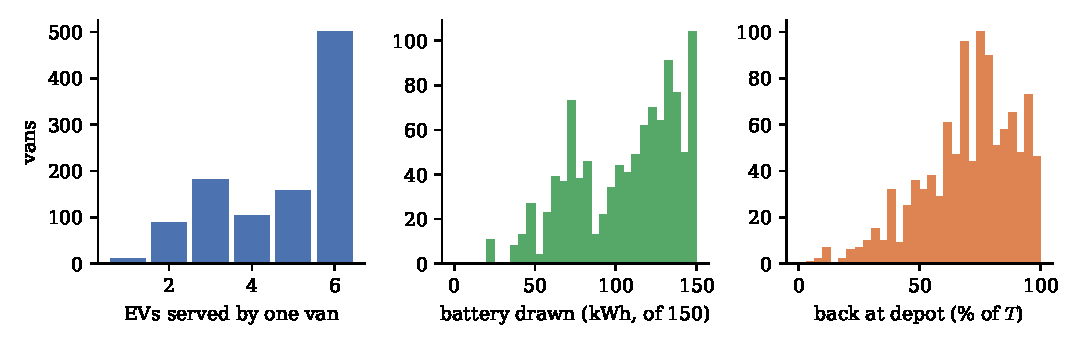
\includegraphics[width=0.95\textwidth]{figures/vans.pdf}
\caption{EVs per van, battery drawn and return time of every dispatched van.}
\label{fig:vans}
\end{figure}
Van definitions (\texttt{common/infra.py}): fleet use = vans dispatched $/\,5$; seats = stops $/\,6$; battery = kWh drawn $/\,150$ (drawn = delivered$/\eta$ + $\beta\times$km); on the road = (return $-$ departure)$/\,T$ with departure = first start minus the drive from the depot; charging $/\,T$ = kWh delivered $/(30\text{ kW}\times T/60)$, the van's power-capacity use; idle = on-road time neither charging nor driving.
\begin{itemize}
  \item \textbf{Fleet:} \UFleetMean\pct{} of the 5 vans leave per plan on average (\UFleetHundred\pct{} at $n=100$); all 5 leave in \UFleetAll\pct{} of plans.
  \item \textbf{Per dispatched van:} seats \USeatMean\pct, battery \UBattMean\pct, on the road \UOnRoadMean\pct{} of $T$, but charging only \UChargeMean\pct{} of $T$; \UIdleShareMean\pct{} of the on-road time is idle (waiting for the next EV's request).
  \item \textbf{Who fills them:} \VansFull\pct{} of vans are full (6 EVs). \SeatsStranded\pct{} of all van seats are taken by stranded EVs, \SeatsPersFree\pct{} by free-choice personal EVs and only \SeatsCommFree\pct{} by free-choice commercial EVs.
  \item \textbf{What limits them:} seats for \TightSeats\pct{} of vans, time for \TightTime\pct{}, the battery for \TightBatt\pct. The split follows the horizon. In R1 and RC1 (230--240 minutes) the vans are on the road \UOnRoadShort\pct{} of $T$, charge \UChargeShort\pct{} of it, are almost never idle (\UIdleShareShort\pct) and serve only \ShortVanStopsMin--\ShortVanStopsMax{} EVs (seats \USeatShort\pct): they run out of time. In C2, R2 and RC2 they fill \USeatLong\pct{} of their seats but charge only \UChargeLong\pct{} of $T$ and are idle \UIdleShareLong\pct{} of their road time: they run out of seats while waiting between requests.
  \item \textbf{Energy:} of the battery energy drawn, \UVanDelivShare\pct{} reaches the EVs, \UVanLossShare\pct{} is lost in transfer and \UVanDriveShare\pct{} drives the van (the split adds up to the energy drawn of every van to within \UVanEnergyCheck{} kWh).
\end{itemize}

\inshort{Vans are filled first by stranded EVs, then by rich personal owners. Fewer than half of the vans leave; those that do charge only about a quarter of $T$. With a long horizon a van's limit is its 6 seats, and it spends much of its road time waiting; with a short one, its time. The battery is rarely the limit.}

%---------------------------------------------------------------------
\subsection{Money paid and perceived cost: equity across segments}
\label{sec:equity}
\begin{figure}[H]
\centering
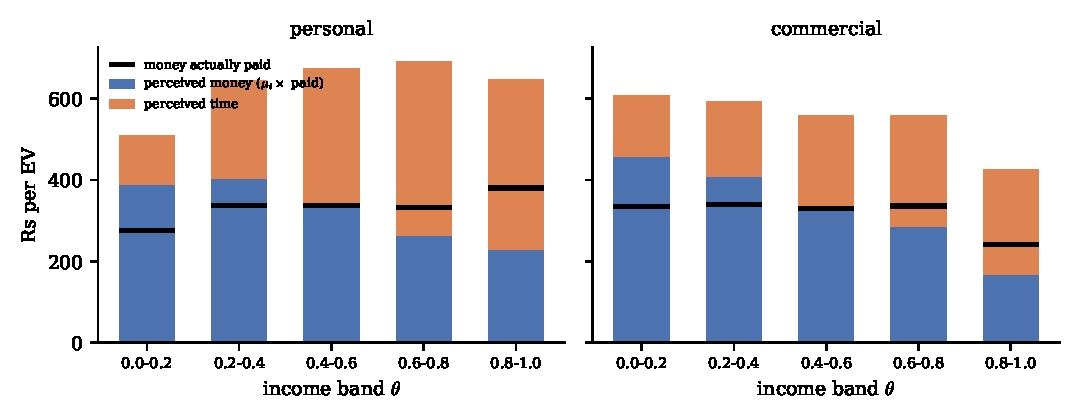
\includegraphics[width=\textwidth]{figures/equity.pdf}
\caption{Money paid and perceived cost per EV by income band, per segment.}
\label{fig:equity}
\end{figure}
\begin{table}[H]
\centering\scriptsize
\caption{Shares of money paid and perceived cost by segment and income band.}
\label{tab:equity}

\resizebox{\textwidth}{!}{\begin{tabular}{lrrrrrrrr}\toprule
segment & income $\theta$ & \shortstack{share of\\EVs (\%)} & \shortstack{share of\\money paid (\%)} & \shortstack{share of\\perceived cost (\%)} & \shortstack{perceived per\\Rs paid} & \shortstack{time share of\\perceived (\%)} & \shortstack{paid per\\kWh (Rs)} & \shortstack{request to\\charged (min)} \\ \midrule
personal & 0.0--0.2 & 0.5 & 0.4 & 0.4 & 1.84 & 23.6 & 15.5 & 58.7 \\
 & 0.2--0.4 & 2.9 & 2.9 & 3.1 & 1.92 & 37.6 & 16.9 & 67.1 \\
 & 0.4--0.6 & 6.3 & 6.2 & 7.0 & 2.00 & 49.9 & 17.1 & 64.2 \\
 & 0.6--0.8 & 8.1 & 7.9 & 9.3 & 2.08 & 62.0 & 17.4 & 61.7 \\
 & 0.8--1.0 & 11.8 & 13.2 & 12.6 & 1.70 & 64.7 & 19.7 & 56.3 \\
commercial & 0.0--0.2 & 10.6 & 10.4 & 10.7 & 1.82 & 24.8 & 16.5 & 71.0 \\
 & 0.2--0.4 & 32.0 & 32.0 & 31.4 & 1.75 & 31.3 & 17.1 & 65.1 \\
 & 0.4--0.6 & 22.5 & 21.9 & 20.8 & 1.69 & 40.4 & 16.9 & 60.8 \\
 & 0.6--0.8 & 5.0 & 4.9 & 4.6 & 1.66 & 48.8 & 17.5 & 61.3 \\
 & 0.8--1.0 & 0.3 & 0.2 & 0.2 & 1.76 & 60.7 & 15.5 & 50.3 \\
\bottomrule\end{tabular}
}
\end{table}
\begin{itemize}
  \item Commercial customers pay \PayShareCommercial\pct{} of the money and carry \PercShareCommercial\pct{} of the perceived cost; personal customers \PaySharePersonal\pct{} and \PercSharePersonal\pct.
  \item Perceived cost per rupee paid is \PercPerRsPersonal{} for personal and \PercPerRsCommercial{} for commercial customers. The composition differs: time is \TimeSharePersonal\pct{} of what personal customers feel (\TimeSharePersTop\pct{} in the richest band) and \TimeShareCommercial\pct{} for commercial ones (\TimeShareCommPoor\pct{} for the poorest commercial band).
  \item Personal owners pay more per kWh (\PaidPerKWhPersonal{} against \PaidPerKWhCommercial{} Rs; \PaidPerKWhPersTop{} Rs in the richest personal band) because they use the dearer van; commercial drivers pay less but are out of service longer: \DowntimeCommPoor{} min for the poorest commercial band against \DowntimeCommMid{} min at $\theta$ 0.4--0.6.
\end{itemize}

\inshort{Each group bears the cost it minds least in rupee terms: rich personal owners pay for the van, poor commercial drivers wait, drive and lose service time.}

%---------------------------------------------------------------------
\subsection{Instance size and computation}
\label{sec:computation}
\begin{table}[H]
\centering\small
\caption{Model size and solver behaviour by instance size (medians over the 56 instances of each size).}
\label{tab:model}
\begin{tabular}{lrrrrrrr}\toprule
$n$ & \shortstack{binary\\variables} & \shortstack{continuous\\variables} & constraints & \shortstack{build\\time (s)} & \shortstack{median\\B\&B nodes} & \shortstack{median gain over\\greedy (\%)} & \shortstack{greedy plan\\found (\%)} \\ \midrule
10 & 807 & 30 & 1,856 & 0.0 & 1 & 0.4 & 98.2 \\
20 & 2,655 & 60 & 6,572 & 0.1 & 1 & 1.2 & 98.2 \\
30 & 5,653 & 90 & 17,248 & 0.4 & 1 & 0.9 & 98.2 \\
40 & 9,712 & 120 & 29,680 & 0.8 & 2,604 & 3.6 & 94.6 \\
50 & 14,672 & 150 & 43,072 & 1.1 & 1,263 & 4.2 & 85.7 \\
60 & 20,945 & 180 & 63,520 & 1.3 & 1,218 & 5.3 & 80.4 \\
70 & 28,191 & 210 & 87,816 & 2.5 & 1,159 & 5.1 & 76.8 \\
80 & 36,445 & 240 & 113,512 & 2.9 & 497 & 5.3 & 67.9 \\
90 & 45,863 & 270 & 143,744 & 3.4 & 1 & 5.6 & 64.3 \\
100 & 56,247 & 300 & 173,514 & 3.4 & 164 & 5.7 & 58.9 \\
\bottomrule\end{tabular}

\end{table}
The model grows quickly: about \BinHundred{} binary variables and \ConsHundred{} constraints at $n=100$, mostly the van arcs $x_{ijm}$ and the pairwise gun-order constraints. The segment adds no variable or constraint. The greedy start plan exists for \GreedyFoundSmall\pct{} of small instances but only \GreedyFoundBig\pct{} at $n=100$; Gurobi improves on it by \GreedyGainMed\pct{} in the median (\GreedyGainBigMed\pct{} for $n\ge50$). The greedy plan used the cost rule in \WarmCost{} instances, the earliest-finish rule in \WarmFinish, and none was found in \WarmNone; the MILP found a valid plan in \ValidNoWarm{} of those.

\inshort{Problem size grows roughly with $n^2$; beyond $n\approx40$ the time limit binds, and the greedy start often fails for large congested instances.}

%---------------------------------------------------------------------
\subsection{Infeasible and unsolved instances}
\label{sec:infeasible}
\begin{table}[H]
\centering\small
\caption{Infeasible instances (Gurobi's verdict) and how many the data test alone proves infeasible.}
\label{tab:infeasible}
\begin{tabular}{lrrrr}\toprule
family & infeasible instances & smallest $n$ & largest $n$ & \shortstack{proven by the\\data test} \\ \midrule
R1 & 29 & 50 & 100 & 29 \\
RC1 & 22 & 10 & 100 & 22 \\
\bottomrule\end{tabular}

\end{table}
\begin{table}[H]
\centering\small
\caption{Unsolved instances (no plan in the time limit) and their demand pressure.}
\label{tab:unsolved}
\begin{tabular}{lrrrr}\toprule
family & \shortstack{unsolved\\instances} & smallest $n$ & \shortstack{mean pressure\\(unsolved)} & \shortstack{mean pressure, solved\\(same family, sizes)} \\ \midrule
C1 & 1 & 100 & 2.01 & 0.35 \\
C2 & 1 & 100 & 1.98 & 0.24 \\
R1 & 16 & 80 & 1.24 & 0.99 \\
RC1 & 16 & 60 & 1.34 & 0.84 \\
RC2 & 1 & 100 & 1.99 & 0.45 \\
\bottomrule\end{tabular}

\end{table}
\begin{itemize}
  \item All \NInf{} infeasible instances are in the short-horizon families \InfFamilies. In \NInfData{} of them the data alone prove it: some EV cannot be charged by $T$ even with a free gun at once or a van leaving the depot at once (test in \texttt{prepare\_data\_f4.py}). Example: \InfExample: EV \InfExampleEV{} requests at minute \InfExampleR; at its nearest station it would finish at minute \InfExampleFinish{} at the earliest, and a van would finish charging at \InfExampleVanEnd{} but be back at the depot only at \InfExampleVanBack, with $T=\InfExampleT$. Segment and income play no role.
  \item The \NNone{} unsolved instances are the most congested ones: their mean demand pressure is \UnsolvedPressure, against \SolvedSamePressure{} for solved instances of the same families and sizes. They need a longer time limit or a better start plan.
\end{itemize}

\inshort{Infeasibility comes from late requests in the short-horizon families, not from the customer model; the unsolved instances are the most congested.}

%---------------------------------------------------------------------
\subsection{Sensitivity to the income distributions and the segment mix}
\label{sec:sensitivity}
The run used Beta(2.5,\,1) for personal and Beta(3,\,5) for commercial incomes and $\pi_{\mathrm C}=\PiC$. If the probability of a van at each income decile stayed as observed in each segment, other distributions would give the van shares below (a reweighting of the decile shares; the plans themselves would adapt, so this is a first-order estimate).
\begin{table}[H]
\centering\small
\caption{Expected van share of free-choice EVs of a segment under other income distributions.}
\label{tab:beta}
\begin{tabular}{lrrr}\toprule
income distribution & mean $\theta$ & EVs with $\theta\ge0.6$ (\%) & expected van share (\%) \\ \midrule
personal: Beta(2.5, 1) (used) & 0.71 & 72.1 & 20.8 \\
personal: Beta(2, 2) (formulation 3) & 0.50 & 35.2 & 6.6 \\
personal: Beta(1, 1) uniform & 0.50 & 40.0 & 10.4 \\
personal: Beta(4, 1) richer & 0.80 & 87.0 & 27.7 \\
commercial: Beta(3, 5) (used) & 0.38 & 9.6 & 0.7 \\
commercial: Beta(2, 2) & 0.50 & 35.2 & 0.4 \\
commercial: Beta(5, 3) richer & 0.62 & 58.0 & 0.1 \\
\bottomrule\end{tabular}

\end{table}
\begin{table}[H]
\centering\small
\caption{Expected van share of all free-choice EVs under other segment mixes (income distributions as used).}
\label{tab:pimix}
\begin{tabular}{lrr}\toprule
commercial share $\pi_{\mathrm{C}}$ & \shortstack{expected van share,\\all free-choice EVs (\%)} & \shortstack{personal share of\\free-choice van users (\%)} \\ \midrule
0.3 & 14.8 & 98.6 \\
0.5 & 10.8 & 96.8 \\
0.7 (used) & 6.7 & 92.9 \\
0.9 & 2.7 & 77.2 \\
\bottomrule\end{tabular}

\end{table}
\begin{itemize}
  \item Personal owners drawn from Beta(2,\,2), as in formulation~3, would get vans \ExpSharePersFThree\pct{} of the time instead of \ExpSharePersonalUsed\pct; a richer population (Beta(4,\,1)) \ExpSharePersRich\pct. Because vans are capacity-limited, the true share would be lower than this estimate at the top.
  \item The commercial income distribution hardly matters (\ExpShareCommercialUsed\pct{} as used, \ExpShareCommRich\pct{} for a richer one): commercial EVs do not get vans at any income.
  \item The segment mix matters most: from $\pi_{\mathrm C}=0.3$ to 0.9 the expected van share of all free-choice EVs falls from \ExpVanPiThree\pct{} to \ExpVanPiNine\pct, because every commercial EV replaces a potential personal van user.
\end{itemize}

\inshort{Who uses vans depends on the share of commercial EVs and on the incomes of personal owners; calibrating $\pi_{\mathrm C}$ and the personal income distribution matters more than the commercial one.}

%---------------------------------------------------------------------
\subsection{Robustness and caveats}
\label{sec:caveats}
\begin{itemize}
  \item \textbf{Placeholder parameters.} Directions come from the formulation, sizes from the placeholder lines; the elasticity and tornado tables show which ones matter.
  \item \textbf{Time-limit plans.} Valid but not proven optimal; they contain artefacts such as commercial and low-income van users with long waits. Every segment result is checked on the proven-optimal plans.
  \item \textbf{Unsolved instances.} The most congested instances are missing, so the analysis under-represents extreme congestion, exactly where commercial EVs might take vans.
  \item \textbf{Shadow prices are conditional} on the plan's decisions; values of discrete resources need re-solving (experiments E2, E8).
  \item \textbf{Demand pressure is a proxy}: it ignores travel time and counts a van as one charger.
  \item \textbf{Attributes are independent of location}: richer and poorer neighbourhoods, taxi stands and residential areas are not modelled; $s_i$ and $\theta_i$ are drawn independently of where the EV is.
  \item \textbf{One commercial downtime line.} Owner-drivers and fleet cars are pooled in one line $\omega(\theta)$; a fleet with dedicated depot chargers would behave differently.
\end{itemize}

%---------------------------------------------------------------------
\subsection{Calibration and extensions}
\label{sec:calibration}
Sources behind the calibrated numbers and those that could replace the placeholders (\texttt{data/calibration.md}):
\begin{itemize}
  \item \textbf{Segment share.} Cabs are about 10\pct{} of e-car registrations (Vahan, CY 2024); with five times the daily distance and five times the share of public charging, they are about 0.74 of public charging requests, rounded to $\pi_{\mathrm C}=0.70$.
  \item \textbf{Income of personal owners.} Car ownership by urban consumption quintile (HCES 2022--23) gives Beta(2.5,\,1); EV owners are probably richer still.
  \item \textbf{Income of commercial drivers.} App-based cab drivers' net earnings (PAIGAM/IFAT 2024; CIS Mumbai) place a driver household around the 25th--50th urban percentile: Beta(3,\,5). This is the least supported number and the first to replace.
  \item \textbf{Downtime rate.} The placeholder line (about 90--360 Rs per hour of lost contribution) could be replaced by fleet operators' revenue per vehicle-hour.
  \item \textbf{Extensions.} Re-solve with $\pm$ parameters to obtain the discrete shadow prices (one more van, gun or seat; experiments E2, E8); correlate segment and income with location; give fleets a depot-charging option; price van slots differently by segment.
\end{itemize}

%=====================================================================
\section{Summary of findings}
\begin{enumerate}[itemsep=2pt]
  \item The run is sound: \NValid{} valid plans (\NOpt{} optimal); all \NInf{} infeasible instances are infeasible because of the data.
  \item The segment decides who can get a van, income decides who does: personal EVs above a threshold near $\theta^{*}=\ThetaStarP$ get vans, as the formulation predicts; commercial EVs get none in optimal plans, because a taxi gains no driver-free time and the van premium always outweighs the downtime it saves unless the station queue is very long.
  \item Vans leave for stranded EVs; their spare seats go to rich personal owners. Seats limit vans in long horizons, time in short ones.
  \item Commercial and low-income customers absorb the queues and drive farther; at peak, segment and income buy queue priority rather than a van.
  \item Shadow prices: gun-minutes cost \GunMean{} Rs when scarce, paid mostly by commercial drivers waiting behind personal ones; patience limits and the deadline have zero marginal value for fixed plans; one more kW of station power is worth about \DPFmean{} Rs per instance.
  \item The objective is most sensitive to the station tariff, the money sensitivity of low-income commercial drivers and the grid price; the personal threshold is most sensitive to the van tariff, the value of charging time of rich personal owners and the van energy price.
  \item Utilisation is low on average and high at the peak: guns are busy \UGunMean\pct{} of the period and \UIdleGunsMean{} of 24 stay unused per plan, the system uses \USystemMean\pct{} of its installed power, and vans leave in fewer than half of the fleet slots; congestion comes from short bursts, not from too little capacity overall.
  \item The segment mix and the personal income distribution change the van share strongly; they are the calibration inputs that matter most.
\end{enumerate}

{\small Generated from \texttt{baseline\_MILP/results} (\texttt{runs.csv}, \texttt{plan.csv}) and the formulation-4 data by \texttt{prepare\_data\_f4.py} (analysis tables, fixed-plan LP duals) and \texttt{make\_milp\_report.py} (figures, tables, numbers) in this folder.}

\end{document}
